\documentclass[conference]{IEEEtran}

\usepackage{cite}
\usepackage{amsmath,amssymb,amsfonts}
\usepackage{algorithmic}
\usepackage{graphicx}
\usepackage{textcomp}
\usepackage{xcolor}
\usepackage{multirow}
\usepackage{bm}
\usepackage{booktabs}

\graphicspath{{../figure/浠跨湡鍥?}{../figure/绯荤粺妯″瀷妗嗗浘/}{../figure/淇″彿澶勭悊娴佺▼鍥?}{../figure/甯х粨鏋勫浘/}{../figure/鍗槦鍦烘櫙绀烘剰鍥?}}

\def\BibTeX{{\rm B\kern-.05em{\sc i\kern-.025em b}\kern-.08em
    T\kern-.1667em\lower.7ex\hbox{E}\kern-.125emX}}

\begin{document}

%%=========================================================================
%%  TITLE & AUTHORS
%%=========================================================================
\title{DD-Domain Pilot Design for OTFS-Based Integrated Sensing and Communication in LEO Non-Terrestrial Networks}

\author{
\IEEEauthorblockN{Baoshun Liu}
\IEEEauthorblockA{School of Information and Communication Engineering, \\
Beijing University of Posts and Telecommunications, Beijing, China \\
Email: 2025141467@bupt.cn}
}

\maketitle

%%=========================================================================
%%  ABSTRACT
%%=========================================================================
\begin{abstract}
This paper proposes a delay-Doppler (DD) domain pilot framework for orthogonal time frequency space (OTFS) based integrated sensing and communication (ISAC) in low Earth orbit (LEO) non-terrestrial networks (NTN). A single impulse pilot with a rectangular guard region is embedded in the DD grid to support both data transmission and navigation parameter extraction. To address the extreme Doppler of LEO channels, ephemeris-assisted Doppler pre-compensation is introduced, reducing the pilot overhead from a geometrically infeasible design to below one percent. A simplified three-bin fractional interpolator together with fractional-aware pilot cancellation is adopted to improve sub-bin delay and Doppler estimation. Simulations under the 3GPP NTN-TDL-C channel show that OTFS-Ideal outperforms OFDM and OFDM-SIC in the high-SNR regime, while OTFS-Pilot preserves a substantial portion of this gain and achieves sensing performance with an approximately CRB-parallel trend and robustness to moderate ephemeris errors.
\end{abstract}

\begin{IEEEkeywords}
OTFS, integrated sensing and communication, LEO satellite, non-terrestrial network, delay-Doppler domain, channel estimation
\end{IEEEkeywords}

%%=========================================================================
%%  I. INTRODUCTION
%%=========================================================================
\section{Introduction}

Low Earth orbit (LEO) satellite communication is a key enabler for ubiquitous connectivity in sixth-generation (6G) networks. Since Release~17, the 3rd Generation Partnership Project (3GPP) has standardized non-terrestrial network (NTN) support in 5G New Radio (NR), including channel models and system design guidelines for satellite links \cite{3gpp_38811, 3gpp_38821}. However, LEO satellites at altitudes of 600--2000~km move at velocities above 7~km/s, producing Doppler shifts of tens of kHz in the S-band. Such extreme Doppler severely degrades conventional orthogonal frequency-division multiplexing (OFDM) through inter-carrier interference (ICI), fundamentally limiting OFDM performance in high-mobility NTN scenarios \cite{wang_ofdm_ici}.

Orthogonal time frequency space (OTFS) modulation has emerged as a promising alternative for high-Doppler channels \cite{hadani2017otfs}. By operating in the delay-Doppler (DD) domain, OTFS converts the time-varying multipath channel into a two-dimensional quasi-static representation in which each path appears as a localized component at its corresponding delay and Doppler indices \cite{raviteja2018interference}. This structure allows OTFS to exploit delay-Doppler diversity and achieve improved bit error rate (BER) performance relative to OFDM in high-mobility environments. Recent studies have also shown the potential of OTFS for LEO satellite communications \cite{otfs_leo_2023, otfs_leo_jsac2025}.

Meanwhile, integrated sensing and communication (ISAC) has been recognized as an important 6G technology that shares spectrum and hardware resources between communication and sensing functionalities \cite{dd_isac_2024}. For LEO NTN systems, the ability to transmit data and extract navigation parameters such as range and relative velocity from the same waveform is attractive for reducing system complexity and spectrum consumption. The DD domain is particularly suitable for ISAC because the channel response directly encodes the physical delay and Doppler of the propagation paths \cite{dd_isac_2024, gaudio2020otfs_radar}.

While prior works have studied OTFS for LEO \cite{otfs_leo_2023, otfs_leo_jsac2025} or DD-ISAC in terrestrial settings \cite{dd_isac_2024, gaudio2020otfs_radar}, the joint pilot-overhead and Doppler pre-compensation design for the extreme LEO Doppler regime has not been fully addressed. The main challenges are:
\begin{enumerate}
  \renewcommand{\labelenumi}{\arabic{enumi})}
  \item The extreme Doppler shift in LEO channels ($\sim$48~kHz at 2~GHz) requires an impractically large Doppler guard ($k_{\mathrm{g}} > M/2$) around the DD pilot if no pre-compensation is applied, rendering the pilot scheme geometrically infeasible.
  \item Fractional delay and Doppler offsets cause inter-bin interference via Dirichlet kernel spreading, degrading both channel estimation and navigation accuracy.
  \item A systematic comparison of OFDM, OTFS, and OTFS-with-pilot schemes under realistic 3GPP NTN channel models is lacking.
\end{enumerate}

In this paper, we address these challenges with the following contributions:
\begin{enumerate}
  \renewcommand{\labelenumi}{\arabic{enumi})}
  \item \textbf{DD-pilot ISAC for LEO NTN:} We extend DD-domain embedded pilots to extract velocity and range from the LoS path, with fractional-aware pilot reconstruction to reduce model mismatch under Dirichlet spreading.
  \item \textbf{Doppler pre-compensation and overhead analysis:} We quantify how LEO Doppler makes DD pilots geometrically infeasible without pre-compensation, and show that ephemeris-based removal reduces overhead below 1\%.
  \item \textbf{Joint communication-sensing validation:} We jointly evaluate BER and sensing RMSE under the 3GPP TR~38.811 NTN-TDL-C channel, including OFDM-SIC, interpolation ablation, ephemeris-error robustness, and elevation-angle sweeps.
\end{enumerate}

The remainder of this paper is organized as follows. Section~II introduces the system model, including OTFS modulation and the LEO NTN channel. Section~III presents the proposed DD-domain ISAC scheme. Section~IV reports the simulation results. Section~V concludes the paper.

%%=========================================================================
%%  II. SYSTEM MODEL
%%=========================================================================
\section{System Model}

We consider a LEO NTN downlink operating in the S-band, as illustrated in Fig.~\ref{fig:scenario}. The satellite transmits an OTFS-modulated signal carrying both communication data and an embedded DD-domain pilot for ISAC.

\begin{figure}[t]
  \centering
  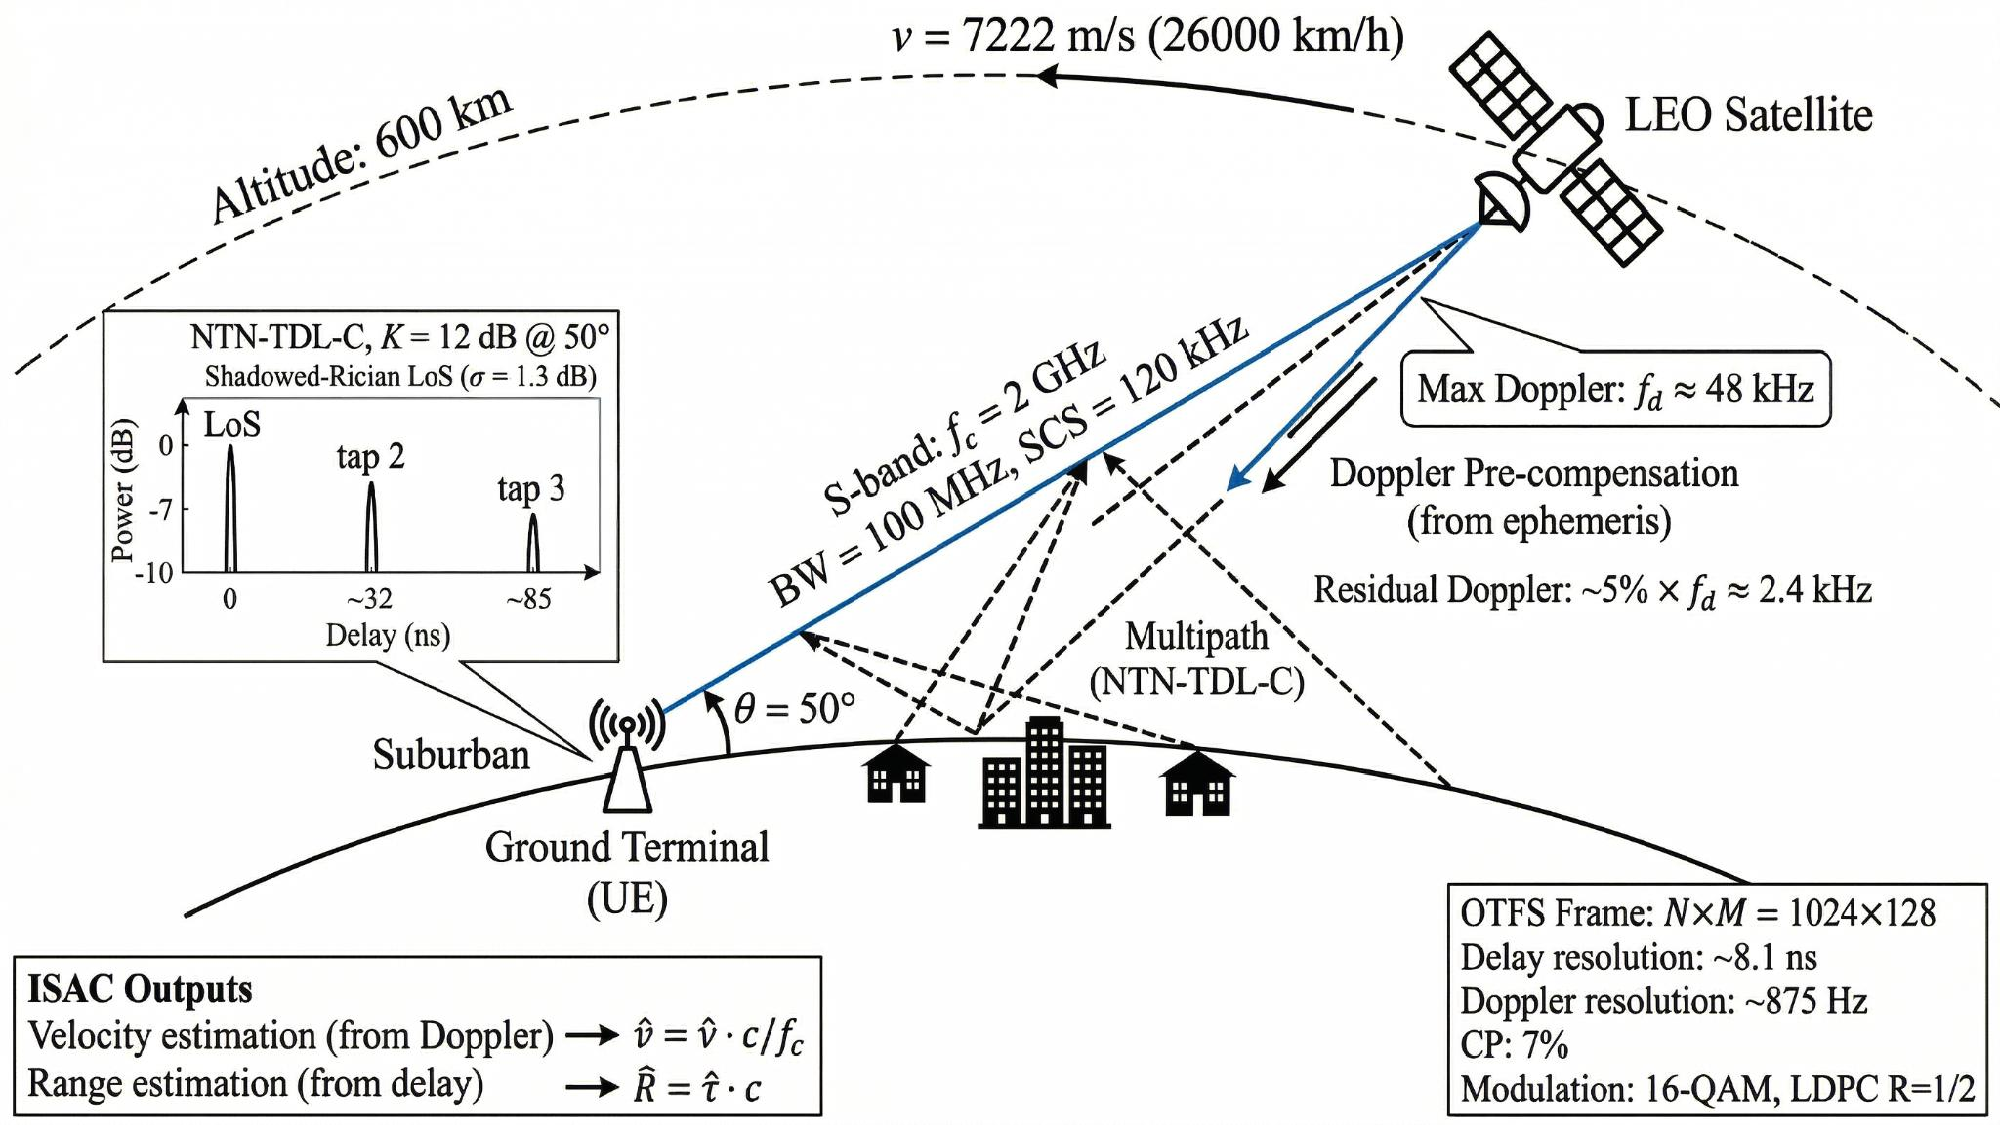
\includegraphics[width=\columnwidth]{../figure/fig1_scenario.pdf}
  \caption{LEO satellite NTN downlink scenario with OTFS-based ISAC. The satellite at 600~km altitude transmits to a ground terminal with Doppler pre-compensation from ephemeris data.}
  \label{fig:scenario}
\end{figure}

\subsection{OTFS Modulation}

The OTFS system uses $N$ subcarriers with spacing $\Delta f$ and $M$ OFDM symbols per frame. The DD grid has resolution $\Delta\tau = 1/(N\Delta f)$ in delay and $\Delta\nu = 1/(M T_{\mathrm{s}})$ in Doppler, where $T_{\mathrm{s}} = (1+\beta)/\Delta f$ is the OFDM symbol duration with cyclic prefix (CP) ratio $\beta$.

Data and pilot symbols are mapped onto the DD grid $\mathbf{X}^{\mathrm{DD}} \in \mathbb{C}^{N \times M}$ and transformed to the time-frequency (TF) domain via the inverse symplectic finite Fourier transform (ISFFT):
\begin{equation}\label{eq:isfft}
  X^{\mathrm{TF}}[n,m] = \frac{1}{\sqrt{NM}} \sum_{l=0}^{N-1} \sum_{k=0}^{M-1} X^{\mathrm{DD}}[l,k]\, e^{j2\pi\!\left(\frac{nl}{N} - \frac{mk}{M}\right)}.
\end{equation}
At the receiver, the TF grid is converted back to the DD domain via the symplectic FFT (SFFT):
\begin{equation}\label{eq:sfft}
  Y^{\mathrm{DD}}[l,k] = \frac{1}{\sqrt{NM}} \sum_{n=0}^{N-1} \sum_{m=0}^{M-1} Y^{\mathrm{TF}}[n,m]\, e^{-j2\pi\!\left(\frac{nl}{N} - \frac{mk}{M}\right)}.
\end{equation}

\subsection{LEO NTN Channel Model}

The channel follows the 3GPP TR~38.811 NTN-TDL-C model \cite{3gpp_38811}, consisting of $P$ paths with delay $\tau_i$, Doppler $\nu_i$, and gain $h_i$. The NTN-TDL-C profile is derived from NTN-TDL-A via Rician K-factor scaling \cite{3gpp_38901}:
\begin{equation}\label{eq:kfactor}
  P_i^{\mathrm{scat}} = \frac{P_i^{\mathrm{base}}}{K + 1}, \quad
  P^{\mathrm{LoS}} = \frac{K}{K + 1},
\end{equation}
where $K$ depends on the elevation angle $\theta_{\mathrm{el}}$ and scenario. At $\theta_{\mathrm{el}} = 50^\circ$ in Suburban, $K \approx 12$~dB.

The LoS path undergoes shadowed-Rician fading (Loo model) \cite{loo_model}:
\begin{equation}\label{eq:los_fading}
  h_1 = \sqrt{\tfrac{K}{K+1}} \cdot 10^{\xi/20} \cdot e^{j\phi_0} + h_1^{\mathrm{scat}},
\end{equation}
where $\xi \sim \mathcal{N}(0, \sigma_{\mathrm{s}}^2)$ models shadow fading with $\sigma_{\mathrm{s}}$ from ITU-R P.681 \cite{itu_p681}, and $\phi_0 \sim \mathcal{U}[0, 2\pi)$.

For a LEO satellite with velocity $v_{\mathrm{sat}}$, the maximum Doppler is $f_{\mathrm{d}} = v_{\mathrm{sat}} f_{\mathrm{c}} / c$. Scatter paths have Doppler $\nu_i = f_{\mathrm{d}} + \delta_\nu \cos(2\pi(i\!-\!1)/P)$ with spread $\delta_\nu = 0.05 f_{\mathrm{d}}$.

\subsection{DD-Domain Input-Output Relation}

The received DD grid is given by a 2D circular convolution:
\begin{equation}\label{eq:dd_io}
  Y^{\mathrm{DD}}[l,k] \!=\! \sum_{i=1}^{P} h_i\, X^{\mathrm{DD}}\!\left[(l \!-\! l_i)_N, (k \!-\! k_i)_M \right] + W[l,k],
\end{equation}
where $l_i = \mathrm{round}(\tau_i / \Delta\tau)$, $k_i = \mathrm{round}((\nu_i - f_{\mathrm{pre}}) / \Delta\nu)$, $f_{\mathrm{pre}}$ is the pre-compensated Doppler, $(\cdot)_N$ denotes modulo-$N$, and $W[l,k]$ is AWGN.

When fractional offsets exist, i.e., $\tau_i/\Delta\tau = l_i + \lambda_i$ and $(\nu_i - f_{\mathrm{pre}})/\Delta\nu = k_i + \kappa_i$ with $\lambda_i, \kappa_i \in [0,1)$, inter-bin spreading occurs \cite{raviteja2019}:
\begin{multline}\label{eq:dd_frac}
  Y[l,k] = \sum_{i=1}^{P} h_i \!\!\sum_{p,q=-N_{\mathrm{s}}}^{N_{\mathrm{s}}} \alpha_p^{(i)} \beta_q^{(i)} \Phi_i[l] \\
  \times\, X\!\left[(l\!-\!l_i\!-\!p)_N,\, (k\!-\!k_i\!-\!q)_M\right],
\end{multline}
where the Dirichlet spreading coefficients are
\begin{equation}\label{eq:spreading}
  \alpha_p^{(i)} \!=\! \frac{1\!-\!e^{j2\pi(\lambda_i - p)}}{N(1\!-\!e^{j2\pi(\lambda_i - p)/N})},\;
  \beta_q^{(i)} \!=\! \frac{1\!-\!e^{j2\pi(\kappa_i - q)}}{M(1\!-\!e^{j2\pi(\kappa_i - q)/M})},
\end{equation}
and $\Phi_i[l] = e^{j2\pi l(k_i + \kappa_i)/(NM)}$ is the phase correction.

%%=========================================================================
%%  III. PROPOSED DD-DOMAIN ISAC SCHEME
%%=========================================================================
\section{Proposed DD-Domain ISAC Scheme}

Fig.~\ref{fig:block_diagram} illustrates the overall transceiver architecture of the proposed scheme, which integrates communication data detection and navigation parameter extraction within a unified OTFS processing chain.

\begin{figure}[t]
  \centering
  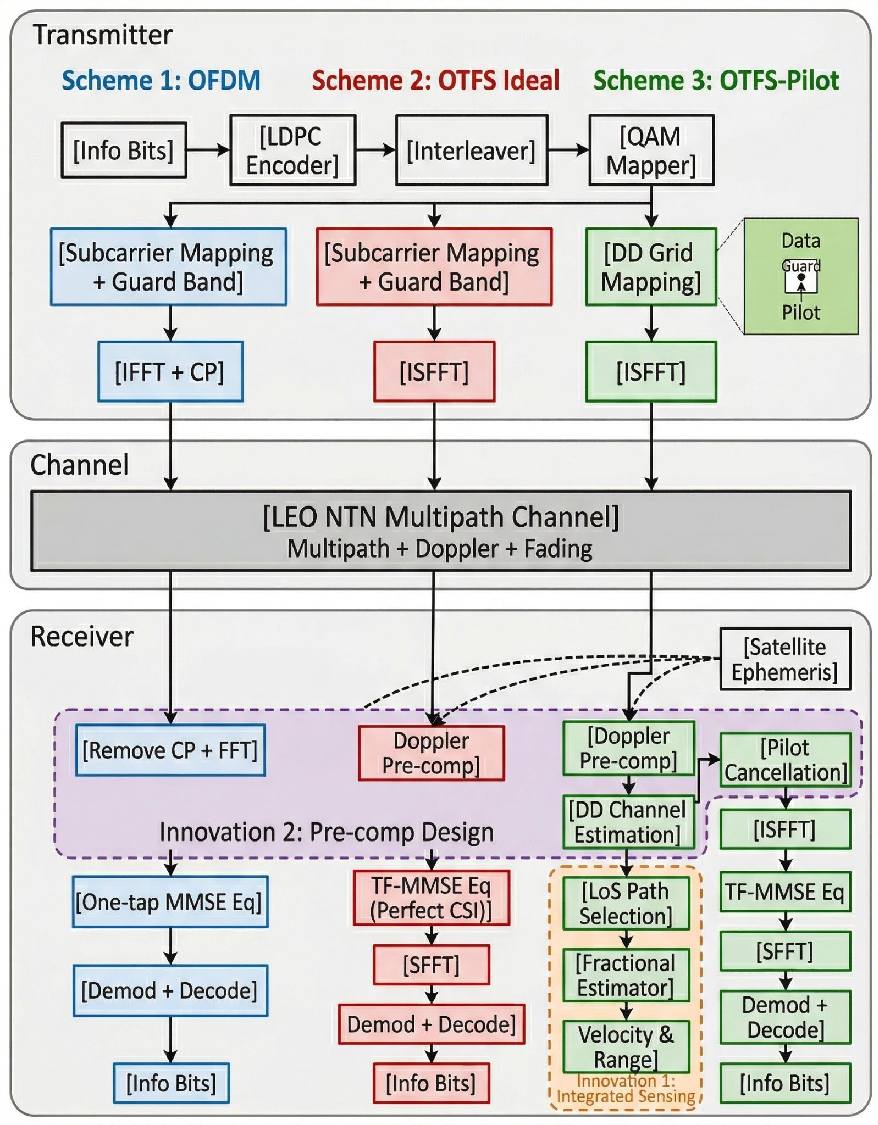
\includegraphics[width=\columnwidth]{../figure/fig2_block_diagram.pdf}
  \caption{Transceiver architecture of the proposed OTFS-based ISAC system, compared with OFDM and OTFS-Ideal baselines. The main design elements are DD pilot-based sensing and ephemeris-assisted Doppler pre-compensation.}
  \label{fig:block_diagram}
\end{figure}

\subsection{DD-Domain Pilot Pattern Design}

As illustrated in Fig.~\ref{fig:frame_structure}, a single high-energy impulse pilot is placed at the center $(l_{\mathrm{p}}, k_{\mathrm{p}})$ of the DD grid and surrounded by a rectangular guard band of size $(2l_{\mathrm{g}}+1) \times (2k_{\mathrm{g}}+1)$. The guard region is zero-padded to prevent data-pilot interference, while data symbols occupy the remaining positions.

\begin{figure}[t]
  \centering
  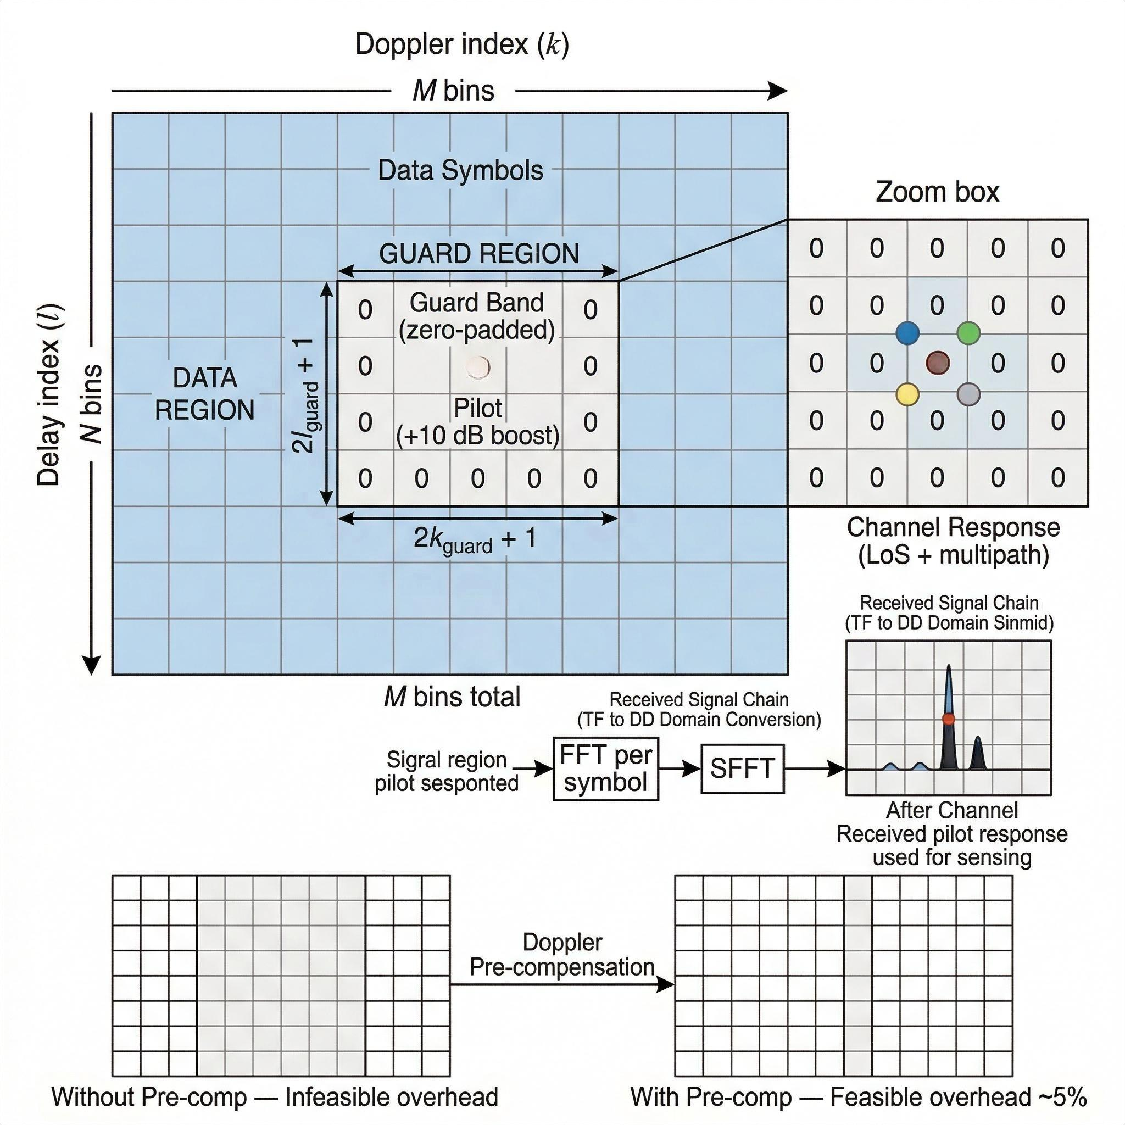
\includegraphics[width=\columnwidth]{../figure/fig3_frame_structure.pdf}
  \caption{DD-domain frame structure with impulse pilot, guard band, and data regions. The guard band size depends on the maximum channel delay spread and residual Doppler after pre-compensation.}
  \label{fig:frame_structure}
\end{figure}
The pilot symbol has a power boost of $P_{\mathrm{boost}}$ dB above the average data power:
\begin{equation}\label{eq:pilot_power}
  x_{\mathrm{p}} = \sqrt{10^{P_{\mathrm{boost}}/10} \cdot \bar{P}_{\mathrm{data}}},
\end{equation}
where $\bar{P}_{\mathrm{data}}$ is the average data symbol power. The total grid power is then normalized to maintain unit average power per active symbol.

\textit{Remark on PAPR:} After ISFFT, the DD-domain pilot impulse is spread across all $NM$ TF elements, with per-element power increment of only $10^{P_{\mathrm{boost}}/10}/(NM) \approx 7.6 \times 10^{-5}$ ($N\!=\!1024$, $M\!=\!128$, $P_{\mathrm{boost}}\!=\!10$~dB), yielding negligible PAPR impact compared to TF-domain pilot boosting.

To fully contain the pilot response including Dirichlet spreading from fractional delay-Doppler offsets, the one-sided guard dimensions are set as $l_{\mathrm{g}} = 2l_{\max}+1$ and $k_{\mathrm{g}} = 2k_{\max}+2$, where $l_{\max} = \lceil \tau_{\max}/\Delta\tau \rceil$ and $k_{\max} = \lceil \nu_{\mathrm{res}}/\Delta\nu \rceil$ are the maximum channel delay and residual Doppler extents in bins, respectively. The factor-of-two margin accounts for the spreading tail of the Dirichlet kernel ($N_{\mathrm{s}} = 2$). The pilot overhead ratio is:
\begin{equation}\label{eq:overhead}
  \eta = \frac{(2k_{\mathrm{g}}+1)(2l_{\mathrm{g}}+1)}{NM}.
\end{equation}

\subsection{Doppler Pre-Compensation and Overhead Analysis}

In LEO NTN, the LoS Doppler $f_{\mathrm{d}}$ can reach about $48$~kHz. Without pre-compensation, $k_{\max} = \lceil f_{\mathrm{d}} / \Delta\nu \rceil = 55$ bins, which requires a one-sided Doppler guard of $k_{\mathrm{g}} = 112$ bins. Because $k_{\mathrm{g}} > \lfloor M/2 \rfloor = 64$, the guard region exceeds the half-grid boundary and the pilot arrangement becomes infeasible, as illustrated in Fig.~\ref{fig:dd_grid}(a).

Since LEO satellite orbits are highly predictable, the ground terminal can obtain the satellite Doppler from broadcast ephemeris data and apply pre-compensation at the transmitter or receiver. After pre-compensation with ratio $\rho \in [0, 1]$, the residual Doppler is:
\begin{equation}\label{eq:residual_doppler}
  \nu_{\mathrm{res}} = (1 - \rho) f_{\mathrm{d}} + \delta_\nu,
\end{equation}
where $\delta_\nu = 0.05 f_{\mathrm{d}}$ accounts for the scatter path spread. The maximum residual Doppler in bins and the required one-sided guard are then:
\begin{equation}\label{eq:kguard}
  k_{\max} = \left\lceil \nu_{\mathrm{res}} / \Delta\nu \right\rceil, \quad
  k_{\mathrm{g}} = 2 k_{\max} + 2,
\end{equation}
and the overhead $\eta$ is computed via (\ref{eq:overhead}). Fig.~\ref{fig:dd_grid} compares the DD grid utilization without and with pre-compensation, demonstrating the critical role of ephemeris-based Doppler removal.

\begin{figure}[t]
  \centering
  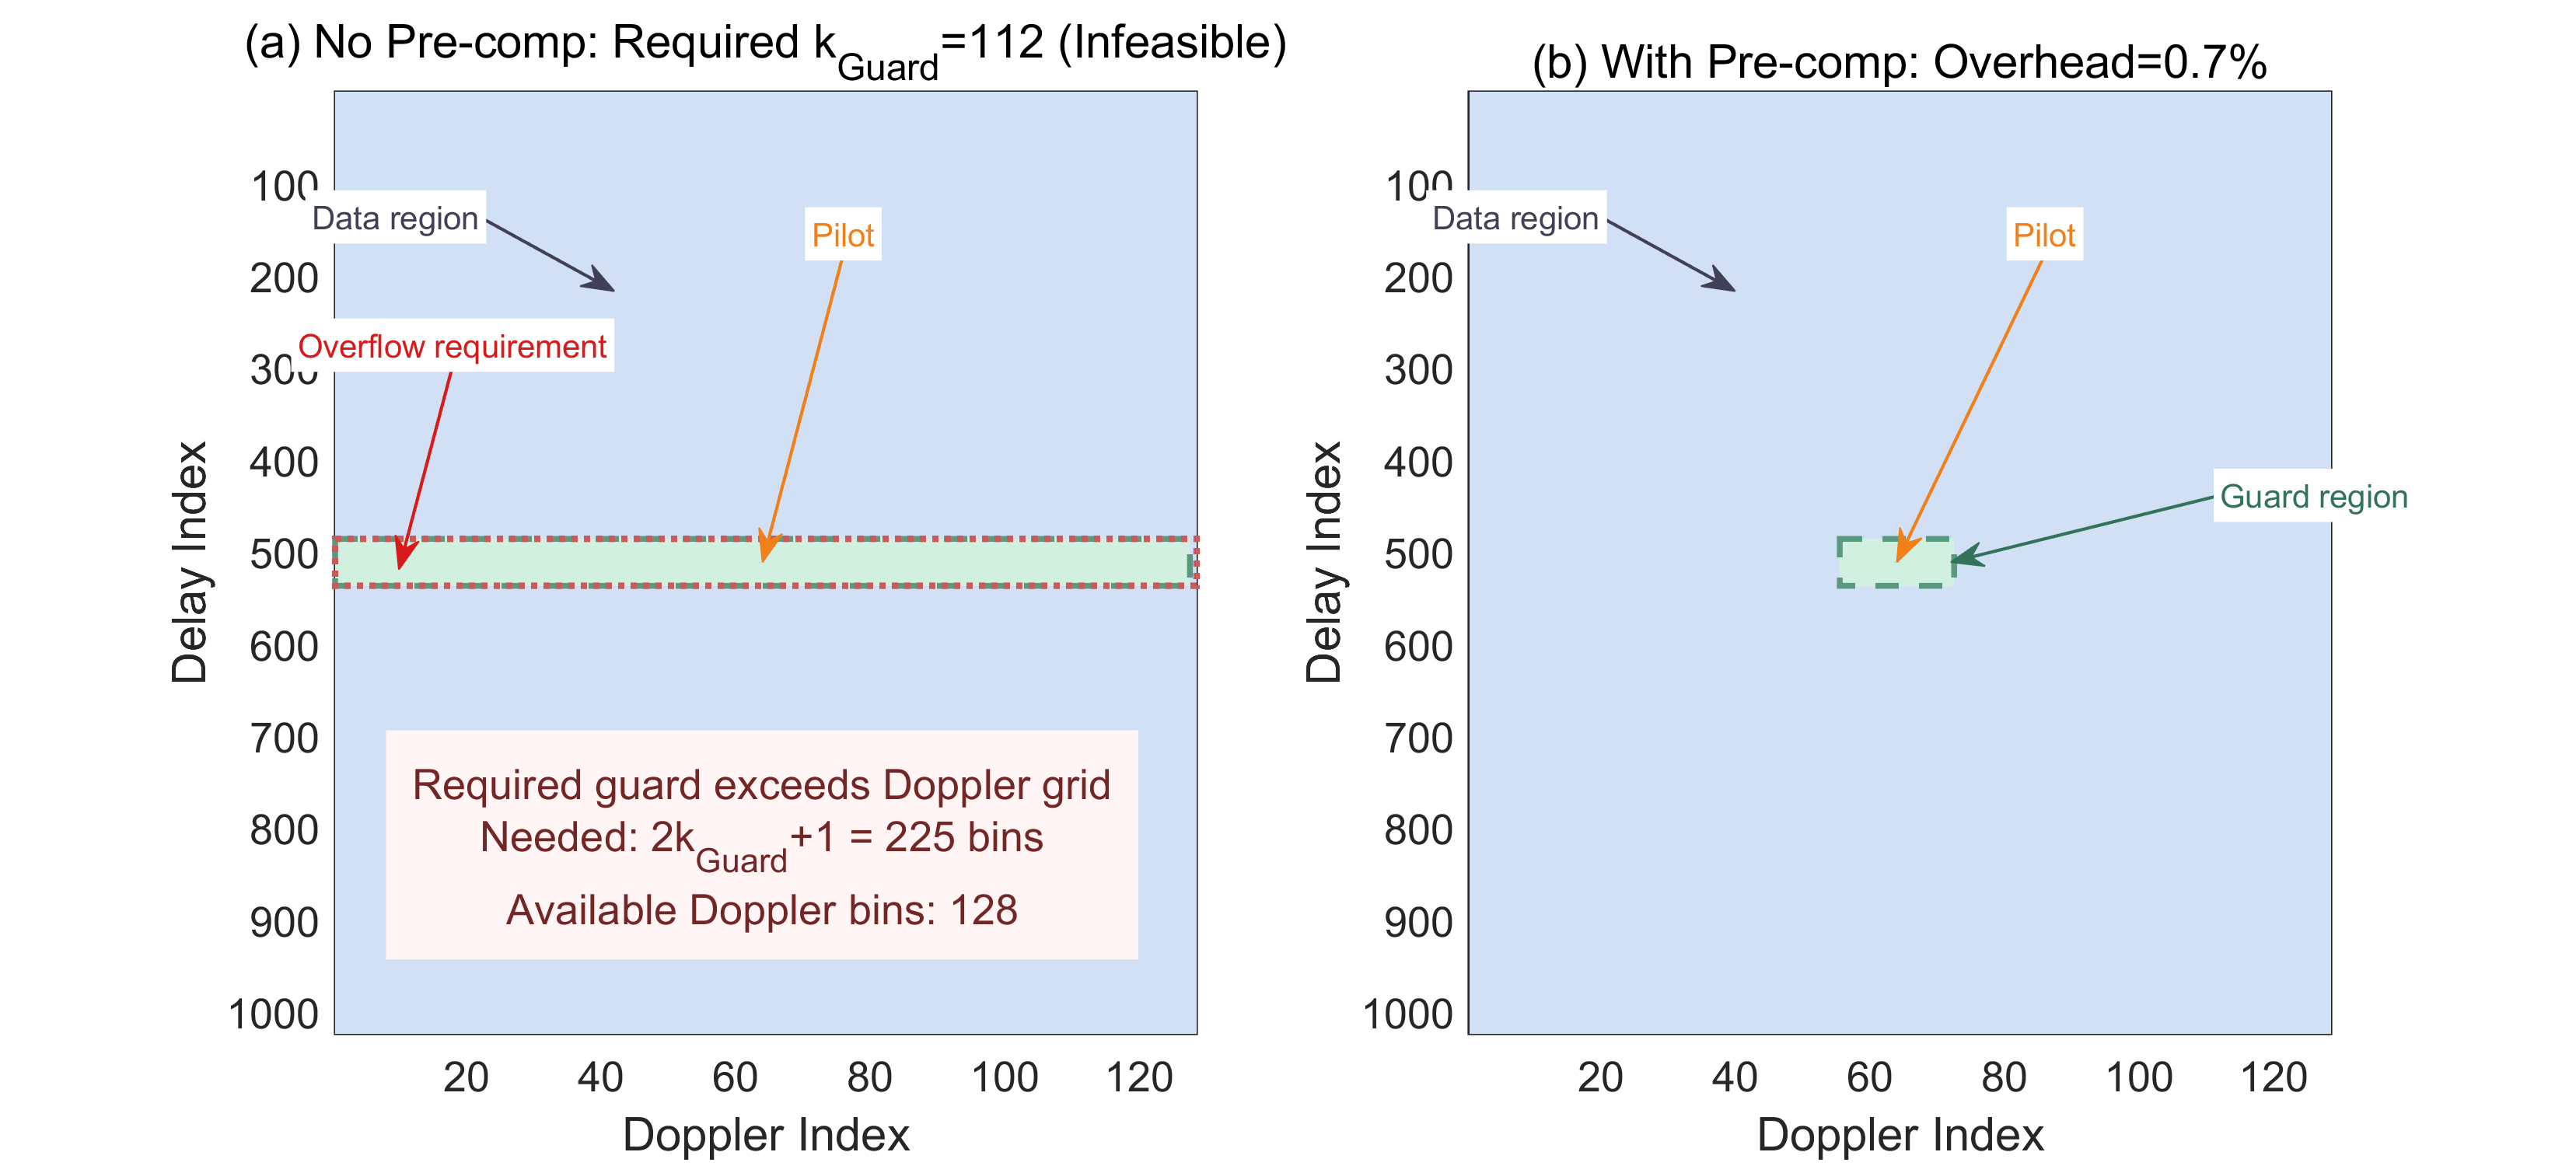
\includegraphics[width=\columnwidth]{../figure/SimulationResult/fig4_dd_grid_pilot_pattern.png}
  \caption{DD grid pilot pattern: (a)~without pre-compensation ($k_{\mathrm{g}} = 112 > M/2$, infeasible); (b)~with pre-compensation ($k_{\mathrm{g}} = 8$, overhead $\approx 0.6\%$).}
  \label{fig:dd_grid}
\end{figure}

\textit{Robustness to ephemeris errors:} Let $\epsilon_{\mathrm{eph}}$ denote the fractional Doppler error, so $\rho = 1 - \epsilon_{\mathrm{eph}}$ and $\nu_{\mathrm{res}} = \epsilon_{\mathrm{eph}} f_{\mathrm{d}} + \delta_\nu$. For GNSS-aided LEO ephemeris, $\epsilon_{\mathrm{eph}} < 0.1\%$ \cite{3gpp_38821}, yielding $\epsilon_{\mathrm{eph}} f_{\mathrm{d}} \approx 48$~Hz $\ll \delta_\nu \approx 2407$~Hz. Hence $k_{\max} = 3$ bins is unchanged and $k_{\mathrm{g}} = 8$ provides a robust margin for ephemeris errors up to $\delta_\nu / f_{\mathrm{d}} = 5\%$ without guard expansion.

\subsection{Channel Estimation and Pilot Cancellation}

After transforming the received signal to the DD domain via SFFT, the channel response appears as shifted copies of the pilot within the guard region. The estimation procedure is as follows.

\textit{1) Path detection:} The guard region is scanned within the physically valid range $l \in [0, l_{\max}]$ and $k \in [-k_{\max}, k_{\max}]$. Paths are detected using the adaptive threshold
\begin{equation}\label{eq:threshold}
  \gamma = \max\!\left(A_{\mathrm{p}} \cdot 10^{-25/20},\; 3A_{\mathrm{n}}\right),
\end{equation}
where $A_{\mathrm{p}}$ is the peak amplitude in the scan region and $A_{\mathrm{n}}$ is an amplitude-domain noise-floor estimate obtained from the median magnitude within the scan region.

\textit{2) Channel gain estimation:} The complex gain of each detected path at relative position $(\Delta l_i, \Delta k_i)$ from the pilot is estimated as
\begin{equation}\label{eq:gain_est}
  \hat{h}_i = Y^{\mathrm{DD}}[l_{\mathrm{p}} + \Delta l_i,\, k_{\mathrm{p}} + \Delta k_i] \,/\, x_{\mathrm{p}}.
\end{equation}

\textit{3) Pilot cancellation:} Instead of cancelling only ideal delta taps, the receiver reconstructs the pilot neighborhood using the detected integer offsets together with the fractional delay/Doppler estimates. In this way, the dominant Dirichlet spreading around each path is removed before data equalization. The cleaned DD grid is
\begin{equation}\label{eq:pilot_cancel}
  \tilde{Y}^{\mathrm{DD}}[l,k] = Y^{\mathrm{DD}}[l,k] - \hat{Y}^{\mathrm{pilot}}[l,k],
\end{equation}
where $\hat{Y}^{\mathrm{pilot}}[l,k]$ denotes the reconstructed fractional pilot response in the guard region.

\textit{4) TF-MMSE equalization:} The cleaned DD grid is transformed to the TF domain via ISFFT. Using the detected DD support, an approximate TF-domain channel for one-tap MMSE equalization is constructed as
\begin{equation}\label{eq:tf_eq}
  \hat{H}[n,m] = \sum_{i} \hat{h}_i \, e^{j2\pi n \Delta l_i / N} \cdot e^{-j2\pi m \Delta k_i / M},
\end{equation}
and MMSE equalization is applied:
\begin{equation}\label{eq:mmse_eq}
  \hat{X}^{\mathrm{TF}}[n,m] = \frac{\hat{H}^{*}[n,m]}{|\hat{H}[n,m]|^2 + \sigma_w^2/\sigma_x^2} \cdot \tilde{Y}^{\mathrm{TF}}[n,m].
\end{equation}
Here, $\sigma_w^2$ denotes the noise power per TF bin and $\sigma_x^2$ denotes the average transmit-symbol power.

\subsection{Navigation Parameter Extraction}

The DD-domain pilot response directly encodes the physical channel parameters, enabling navigation sensing without additional waveform overhead.

\textit{1) LoS path selection:} Among the detected paths within 6~dB of the strongest one, the path with the smallest delay is selected as the LoS component, thereby suppressing scatter reflections and Dirichlet sidelobes.

\textit{2) Fractional estimation:} To achieve sub-bin accuracy, we use a simplified three-bin fractional interpolator based on Quinn-style adjacent-bin ratio estimation \cite{quinn1997} along both delay and Doppler dimensions. For the Doppler dimension, let $\alpha_+ = \mathrm{Re}(X_{+1}/X_0)$ and $\alpha_- = \mathrm{Re}(X_{-1}/X_0)$ be the real-valued ratios of the adjacent bins to the peak $X_0$. The two candidate fractional offsets are
\begin{equation}\label{eq:quinn}
  d_+ = \frac{-\alpha_+}{1 - \alpha_+}, \quad
  d_- = \frac{\alpha_-}{1 - \alpha_-},
\end{equation}
and the unconstrained fractional Doppler estimate is selected as
\begin{equation}\label{eq:doppler_raw}
  \tilde{\delta}_k =
  \begin{cases}
    d_+, & |d_+| < |d_-|, \\
    d_-, & \text{otherwise}.
  \end{cases}
\end{equation}
The final fractional Doppler offset is then clipped to the valid sub-bin interval:
\begin{equation}\label{eq:doppler_clip}
  \delta_k = \max\!\left(-0.5,\; \min\!\left(0.5,\; \tilde{\delta}_k\right)\right).
\end{equation}
An analogous clipped expression is used to obtain the fractional delay offset $\delta_l$.

\textit{3) Velocity and range:} The navigation estimates are:
\begin{align}
  \hat{v} &= (\Delta k_{\mathrm{LoS}} + \delta_k) \cdot \Delta\nu \cdot c / f_{\mathrm{c}} + v_{\mathrm{pre}}, \label{eq:vel_est} \\
  \hat{R} &= (\Delta l_{\mathrm{LoS}} + \delta_l) \cdot \Delta\tau \cdot c, \label{eq:range_est}
\end{align}
where $v_{\mathrm{pre}}$ is the pre-compensated velocity component.

\textit{4) Benchmark Cram\'{e}r-Rao bound:} For a single dominant path observed with AWGN, the reference lower bounds for Doppler- and delay-based estimation are \cite{kay1993}
\begin{align}
  \sigma_v^{\mathrm{CRB}} &= \frac{c}{f_{\mathrm{c}}} \cdot \frac{\sqrt{12}}{2\pi T_{\mathrm{s}} \sqrt{\gamma_{\mathrm{p}} M(M^2-1)}}, \label{eq:crb_vel} \\
  \sigma_R^{\mathrm{CRB}} &= \frac{c\sqrt{12}}{2\pi \Delta f \sqrt{\gamma_{\mathrm{p}} N(N^2-1)}}, \label{eq:crb_range}
\end{align}
where $\gamma_{\mathrm{p}} = 10^{P_{\mathrm{boost}}/10} \cdot \mathrm{SNR}$ is the effective pilot SNR.

%%=========================================================================
%%  IV. SIMULATION RESULTS
%%=========================================================================
\section{Simulation Results}

\subsection{Simulation Setup}

We evaluate the proposed scheme under the system parameters in Table~\ref{tab:params}. Four receivers are compared. The first is \textbf{OFDM} with time-domain ICI and one-tap MMSE equalization. The second is \textbf{OFDM-SIC} with one iteration of time-domain ICI cancellation. The third is \textbf{OTFS-Ideal} with perfect CSI and a DD-domain circular-convolution channel, used as a performance upper bound. The fourth is \textbf{OTFS-Pilot} with the proposed DD pilot-based channel estimation and ISAC processing. Both uncoded 16-QAM and DVB-S.2 LDPC coded ($R = 1/2$, codeword length 64800~bits, belief-propagation decoding with 25 iterations) cases are evaluated. To avoid over-simulating easy SNR points while retaining low-BER reliability, the BER experiment uses adaptive Monte Carlo batching with 50 initial trials, up to 200 trials at high SNR, and a minimum of 100 observed coded-bit errors when possible. The channel is NTN-TDL-C at $50^\circ$ elevation in Suburban with shadowed-Rician LoS fading.

\begin{table}[t]
\centering
\caption{System Parameters}
\label{tab:params}
\renewcommand{\arraystretch}{1.1}
\begin{tabular}{l|l}
\hline
\textbf{Parameter} & \textbf{Value} \\
\hline
Carrier frequency $f_{\mathrm{c}}$ & 2 GHz (S-band) \\
Bandwidth $B$ / Subcarrier spacing $\Delta f$ & 100 MHz / 120 kHz \\
Delay bins $N$ / Doppler bins $M$ & 1024 / 128 \\
Delay res. $\Delta\tau$ / Doppler res. $\Delta\nu$ & 8.14 ns / 876 Hz \\
CP ratio $\beta$ / Modulation & 7\% / 16-QAM \\
Channel coding & DVB-S.2 LDPC, rate $1/2$ \\
LEO altitude / velocity & 600 km / 7.22 km/s \\
Elevation angle / Scenario & $50^\circ$ / Suburban \\
Channel model / K-factor & NTN-TDL-C / 12 dB \\
Max Doppler $f_{\mathrm{d}}$ / Max delay spread & $\sim$48.1 kHz / 90 ns \\
Pilot boost $P_{\mathrm{boost}}$ & 10 dB \\
\hline
\end{tabular}
\end{table}

\subsection{BER Performance Comparison}

Fig.~\ref{fig:ber} shows the BER versus $E_b/N_0$ for the four receivers. The SNR is computed as $\mathrm{SNR} = (E_b/N_0) \cdot R \log_2 M_o \cdot (N_{\mathrm{data}}/N_{\mathrm{total}})$, where $R$ is the code rate, $M_o\!=\!16$, and $N_{\mathrm{data}}/N_{\mathrm{total}}$ accounts for each scheme's guard/DC overhead.

\begin{figure}[t]
  \centering
  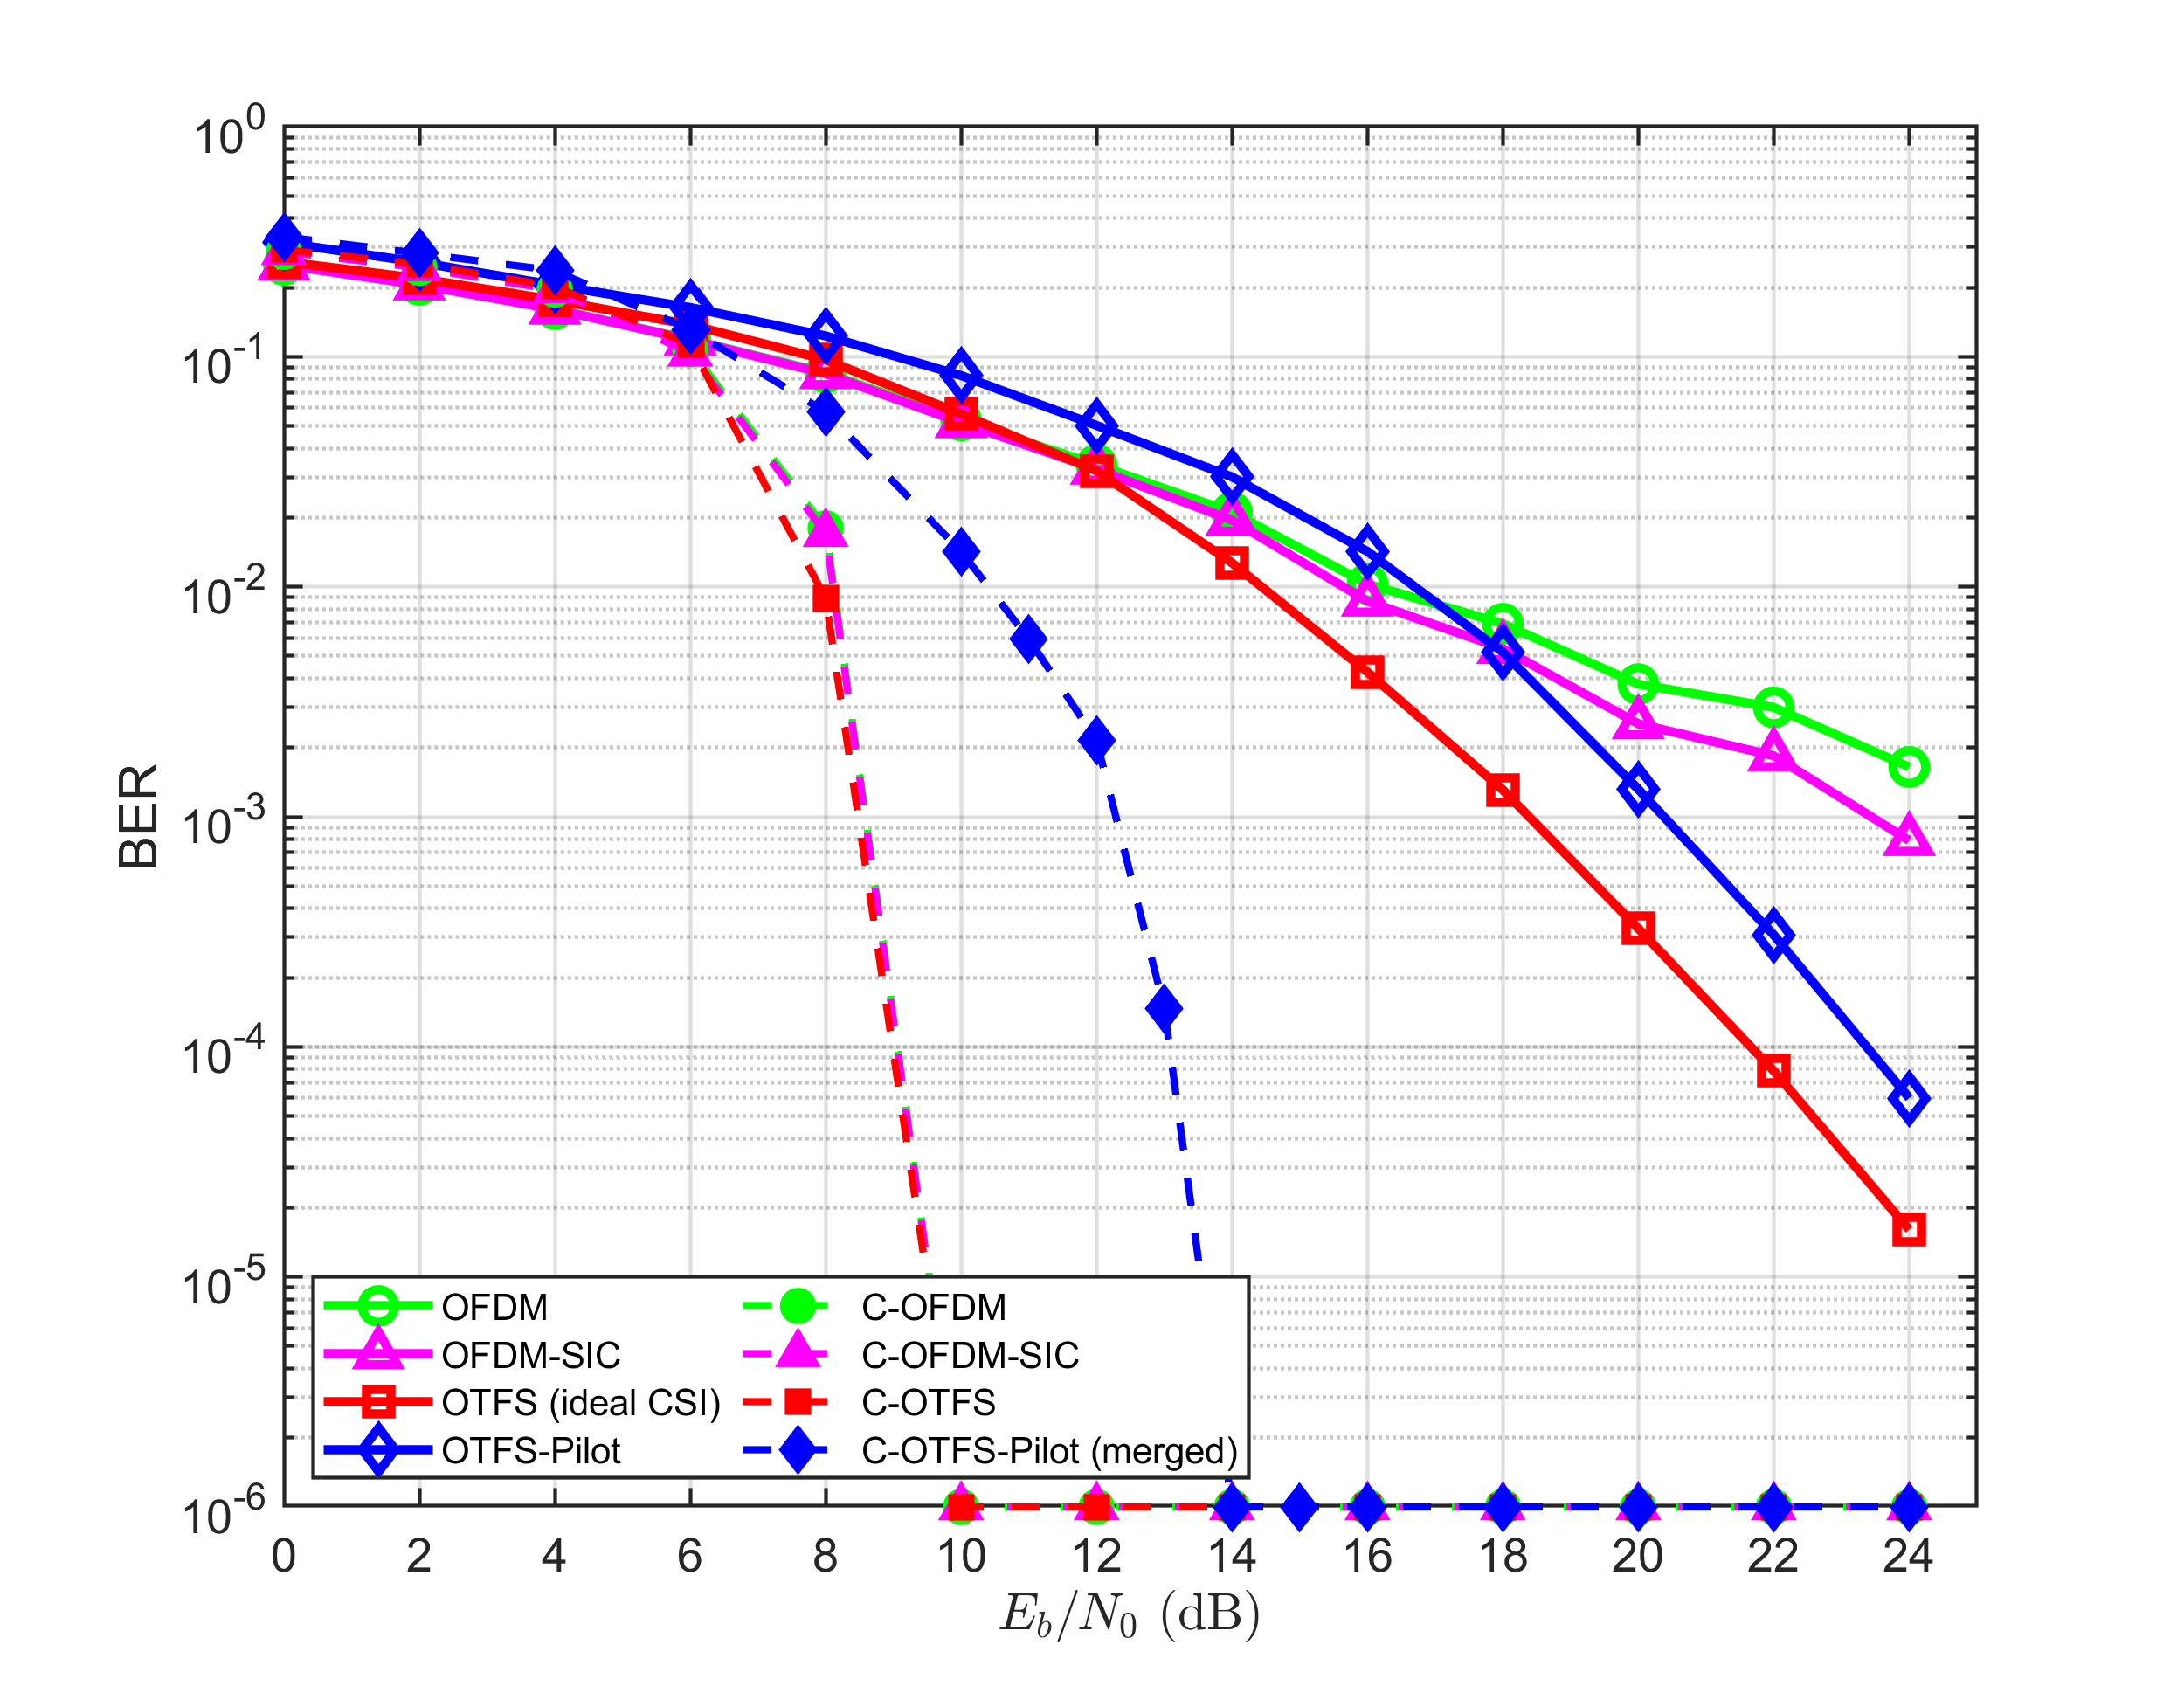
\includegraphics[width=\columnwidth]{../figure/SimulationResult/fig5_ber_comparison.png}
  \caption{BER comparison of OFDM, OFDM-SIC, OTFS-Ideal, and OTFS-Pilot under the NTN-TDL-C channel. Solid: uncoded; dashed: LDPC coded ($R=1/2$).}
  \label{fig:ber}
\end{figure}

Several observations follow from Fig.~\ref{fig:ber}.

\textit{1) OTFS benefits appear mainly in the high-SNR regime:} At $E_b/N_0=20$~dB, the uncoded BER is approximately $3.3\times 10^{-4}$ for OTFS-Ideal, compared with $3.4\times 10^{-3}$ for OFDM and $2.3\times 10^{-3}$ for OFDM-SIC, reflecting the residual ICI penalty of OFDM.

\textit{2) OTFS-Pilot preserves a substantial portion of the OTFS gain:} At $E_b/N_0=20$~dB, the uncoded BER of OTFS-Pilot is about $1.4\times 10^{-3}$, confirming a useful gain over the OFDM baselines with practical channel estimation.

\textit{3) OFDM-SIC yields only a modest improvement:} It improves on plain OFDM, but the gain is limited relative to OTFS-Ideal.

\textit{4) Coded curves should be interpreted as high-level trends:} The rightmost coded points indicate BER below the plotting floor rather than precise ultra-low-BER estimates.

\subsection{Overhead Analysis}

Fig.~\ref{fig:overhead} quantifies the pilot overhead as a function of the Doppler pre-compensation ratio $\rho$.

\begin{figure}[t]
  \centering
  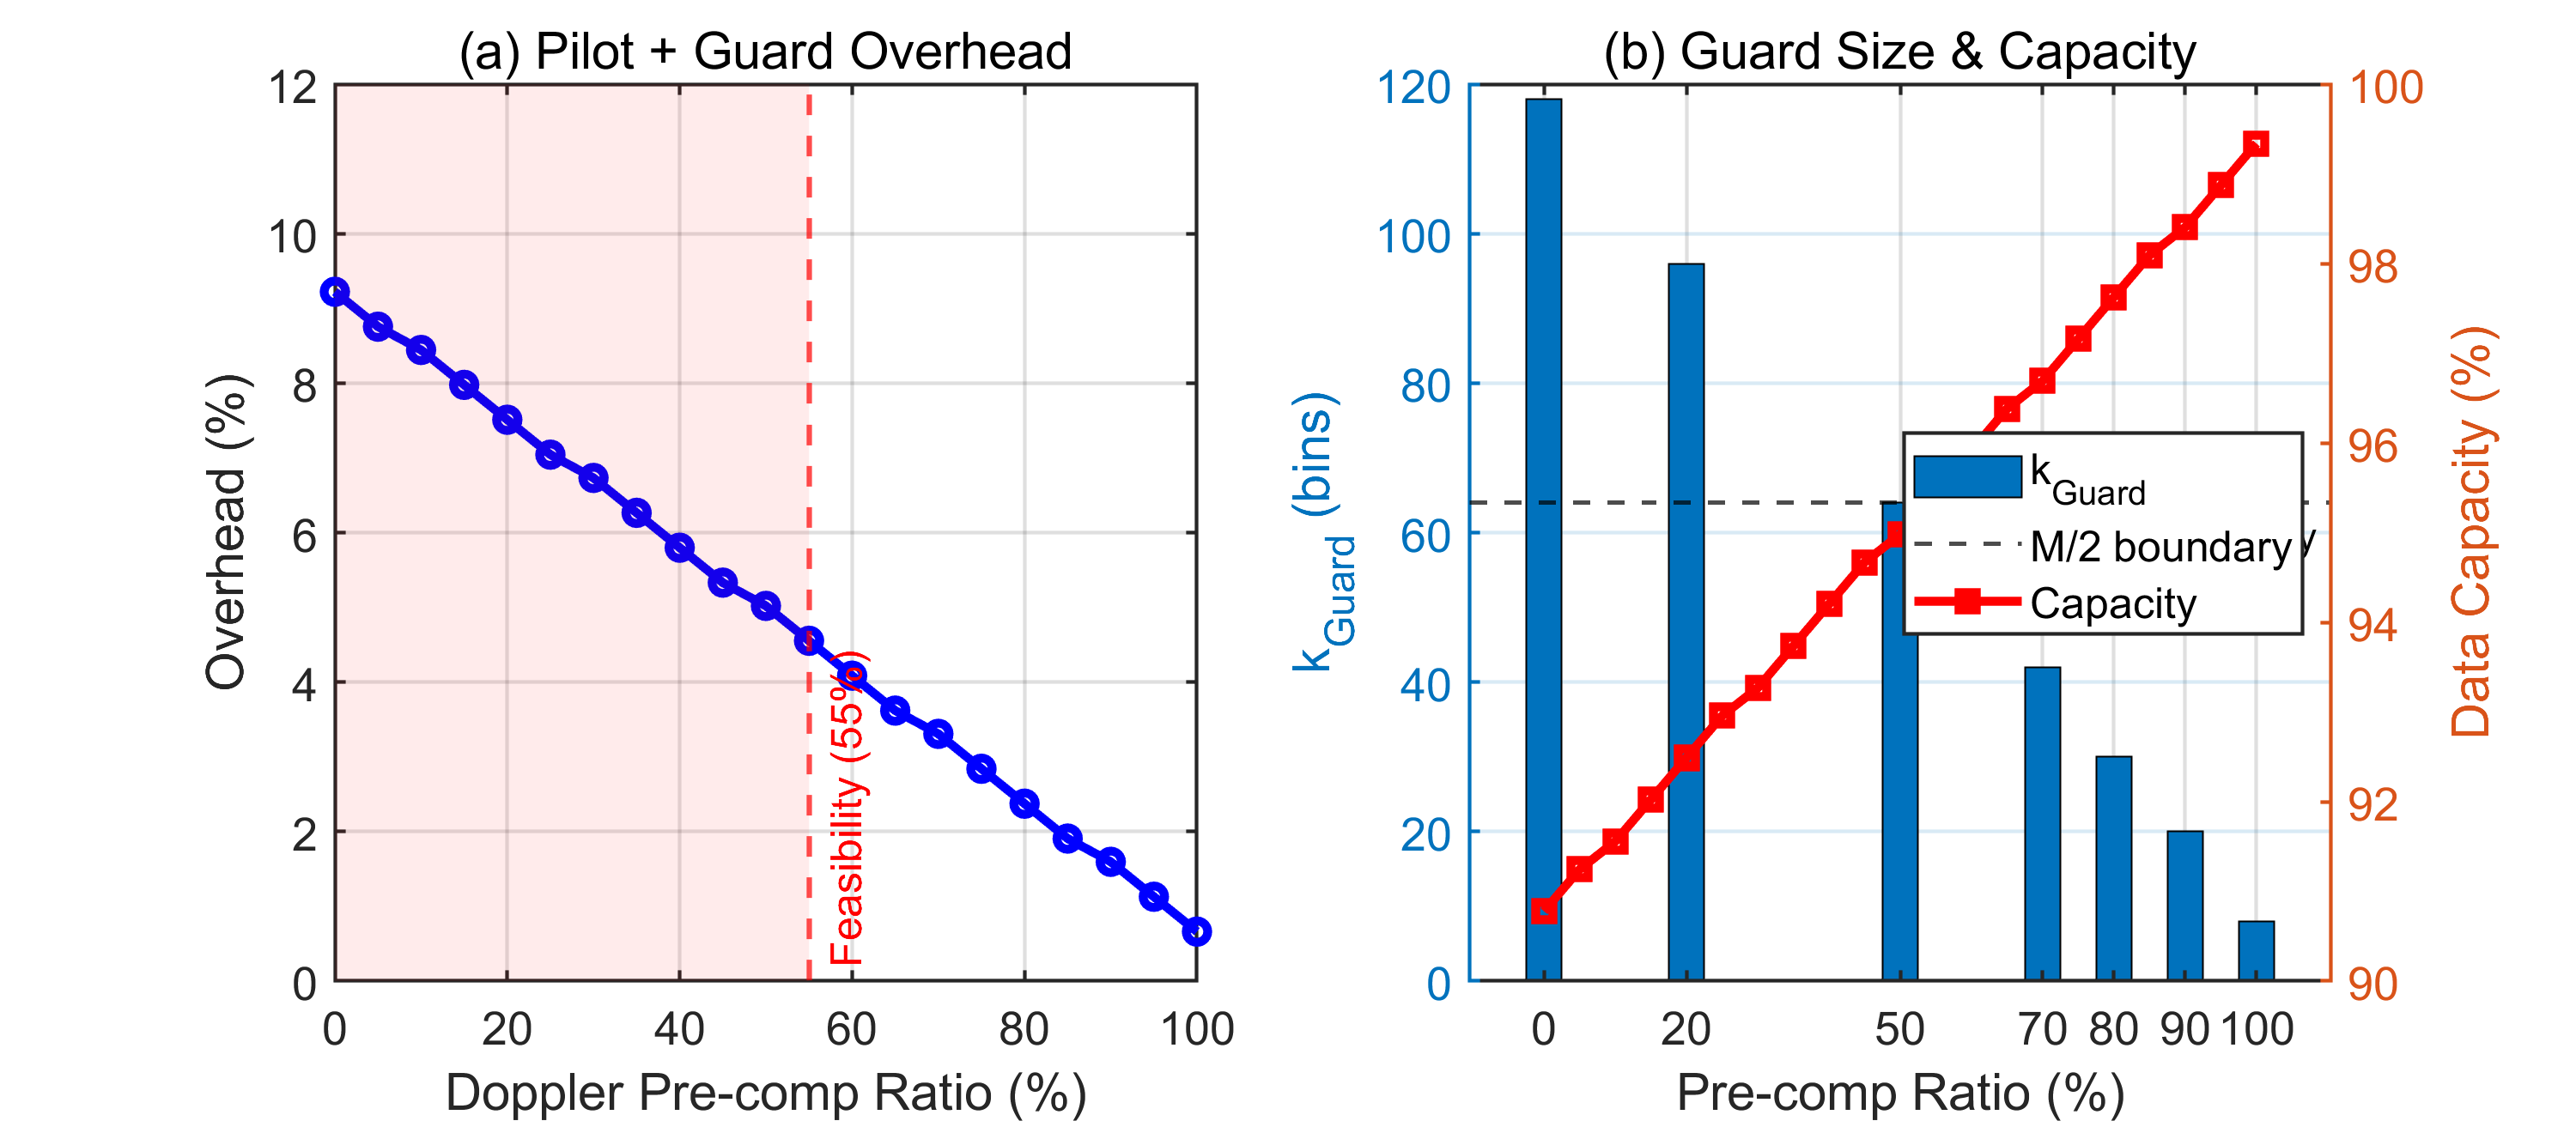
\includegraphics[width=\columnwidth]{../figure/SimulationResult/fig6_overhead_analysis.png}
  \caption{Pilot overhead analysis: (a)~overhead percentage vs.\ pre-compensation ratio with feasibility region; (b)~Doppler guard width and data capacity.}
  \label{fig:overhead}
\end{figure}

As shown in Fig.~\ref{fig:overhead}(a), without pre-compensation ($\rho = 0$), $k_{\mathrm{g}} = 112 > M/2 = 64$ and the pilot scheme is geometrically infeasible (shaded red), with a notional guard overhead of about $9.2\%$. Feasibility begins at approximately $\rho=55\%$. At $\rho = 70\%$ the overhead is about $3.3\%$, and at $\rho = 100\%$, $k_{\max} = 3$, $k_{\mathrm{g}} = 8$, yielding about $0.66\%$. Fig.~\ref{fig:overhead}(b) shows the corresponding $k_{\mathrm{g}}$ and data capacity, confirming that ephemeris-based pre-compensation is essential for practical DD-domain ISAC in LEO NTN.

\subsection{Navigation Accuracy and Ablation}

Fig.~\ref{fig:nav} presents the velocity and range estimation RMSE, computed from the median squared error for robustness to outliers, versus $E_b/N_0$ using 300 Monte Carlo trials.

\begin{figure}[t]
  \centering
  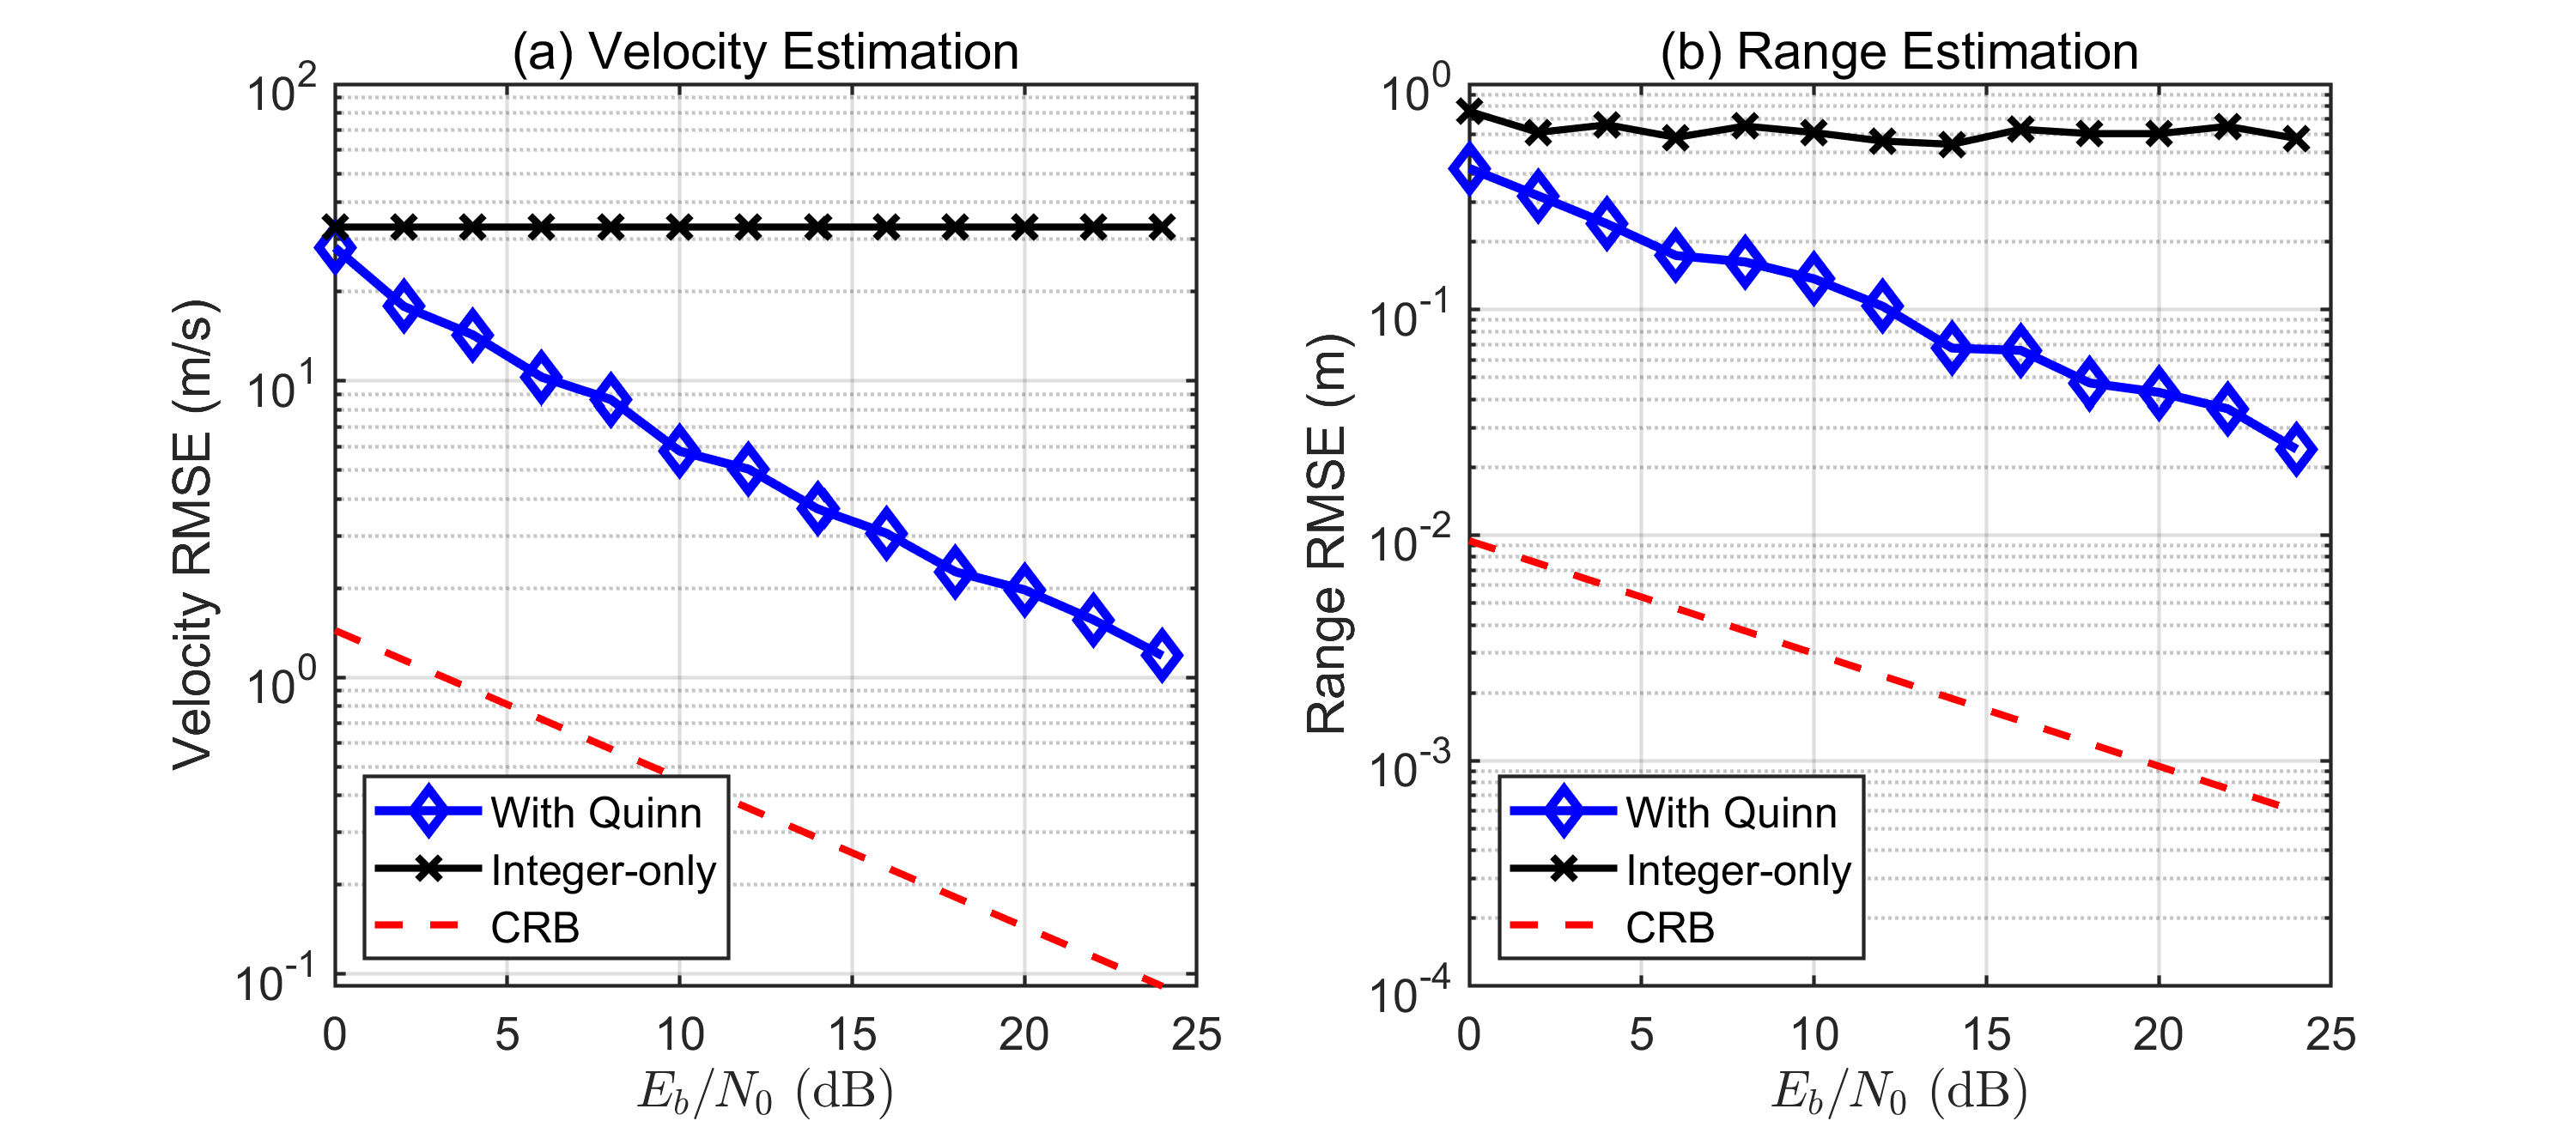
\includegraphics[width=\columnwidth]{../figure/SimulationResult/fig7_navigation_accuracy.png}
  \caption{Navigation accuracy of the proposed OTFS-Pilot ISAC scheme with and without fractional interpolation: (a)~velocity RMSE; (b)~range RMSE. Both are compared against the CRB.}
  \label{fig:nav}
\end{figure}

The velocity RMSE with fractional interpolation decreases from about $28.5$~m/s at $E_b/N_0 = 0$~dB to about $1.2$~m/s at 24~dB, while the range RMSE decreases from about $0.41$~m to about $0.029$~m. In contrast, the integer-only baseline exhibits a clear error floor of about $33$~m/s for velocity and $0.58$--$0.68$~m for range, confirming that sub-bin estimation is essential.

The fractional-interpolation curves remain approximately parallel to the CRB trend, indicating the expected SNR scaling despite a non-negligible gap caused by shadowed-Rician fading, scatter sidelobes, and finite spreading truncation.

\subsection{Robustness to Ephemeris Error}

\begin{figure}[t]
  \centering
  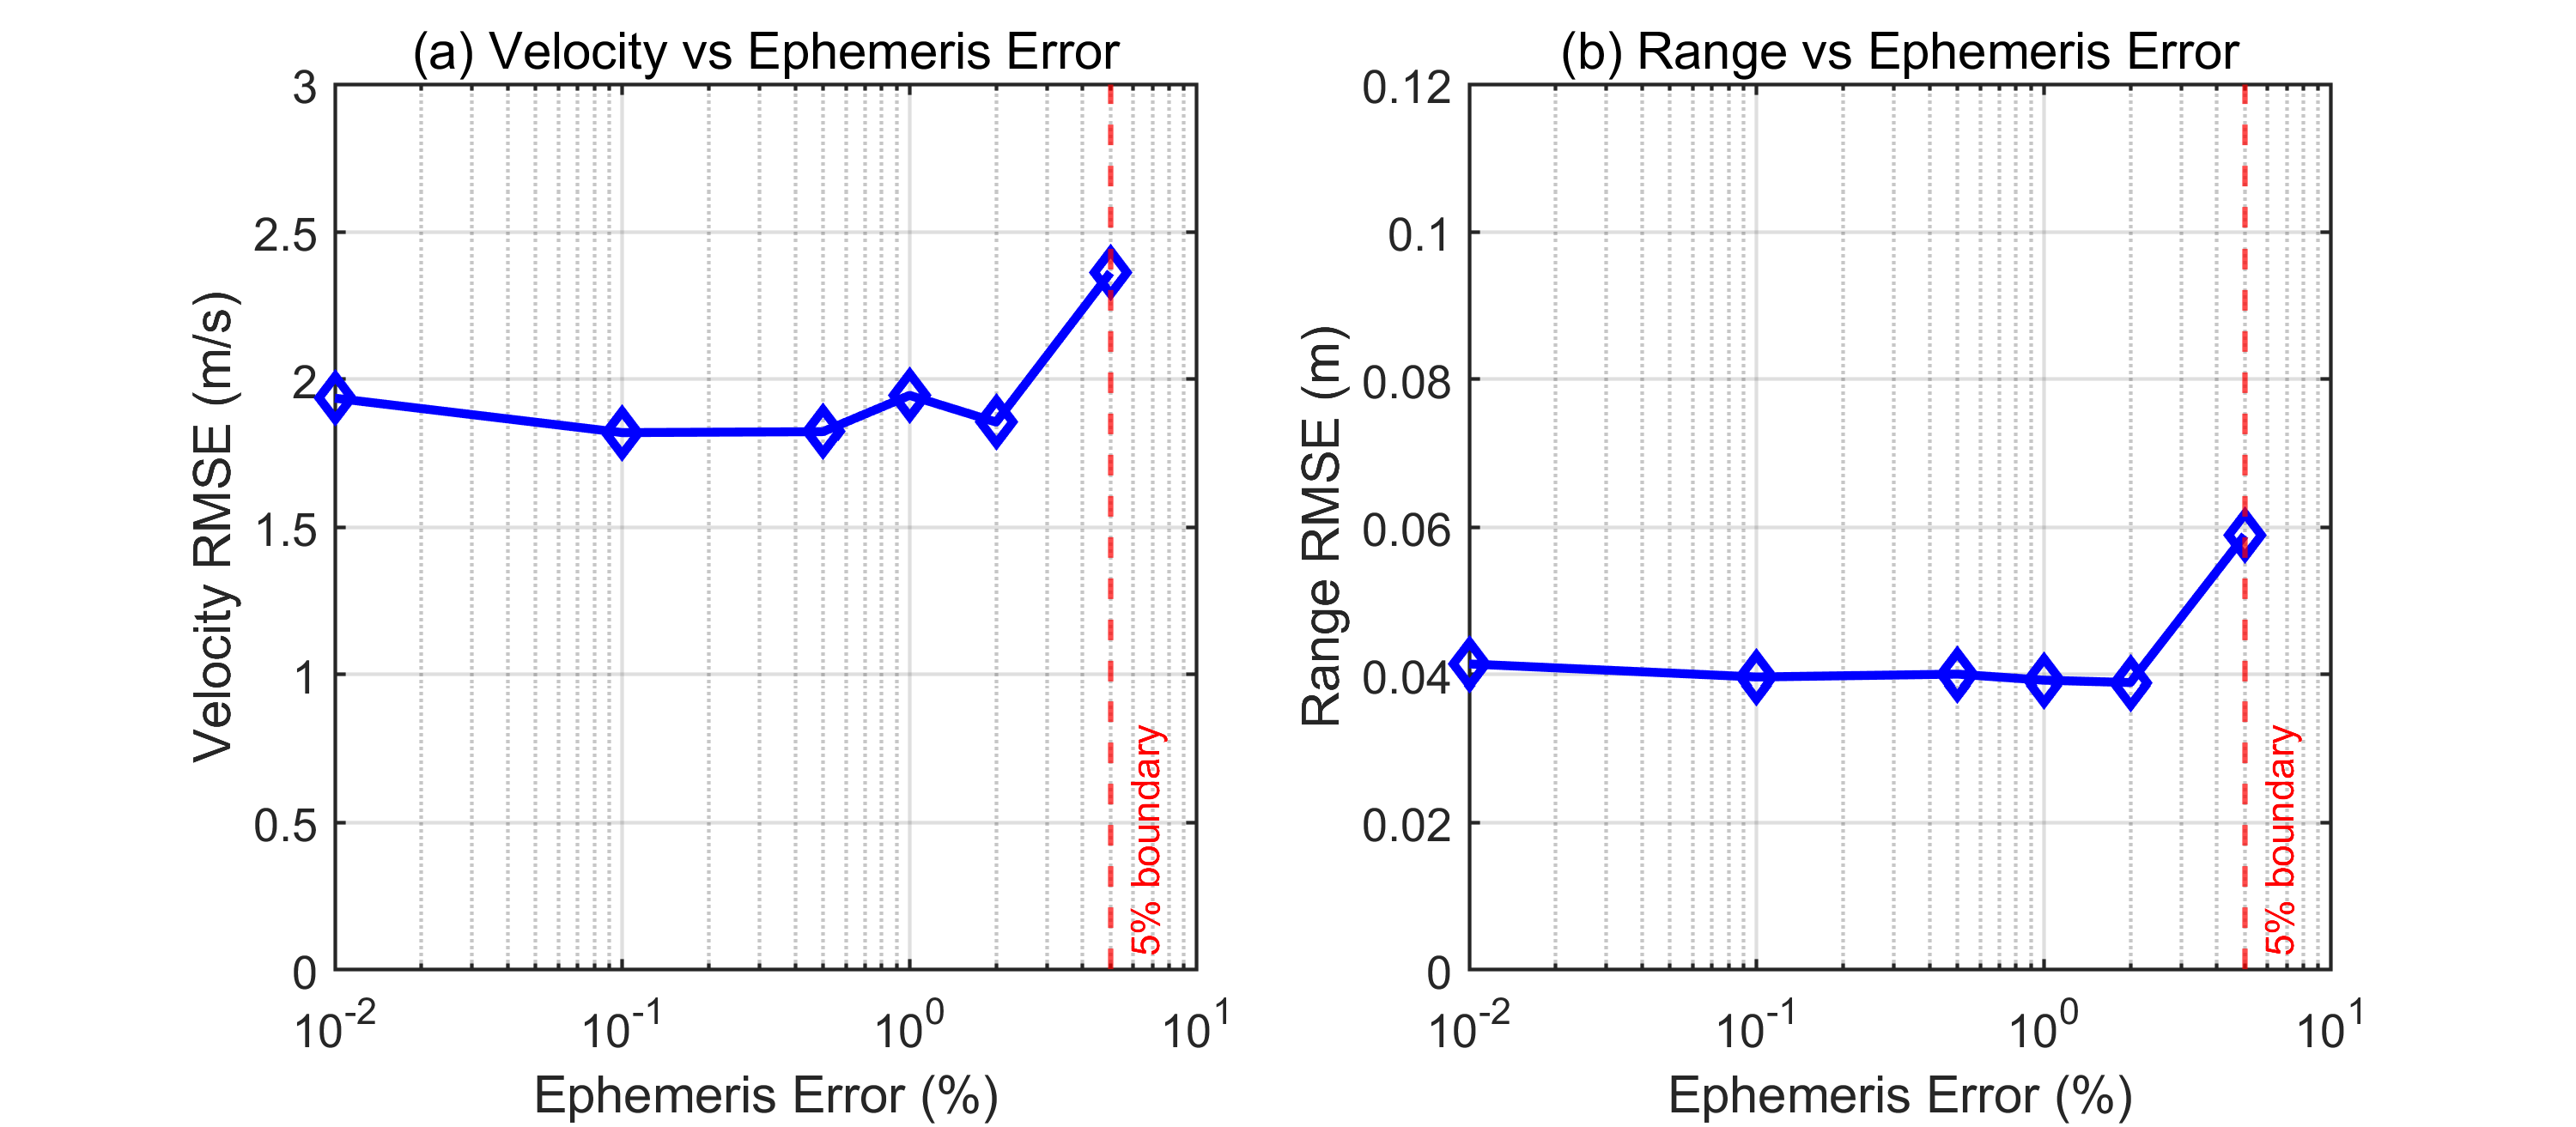
\includegraphics[width=\columnwidth]{../figure/SimulationResult/fig8_ephemeris_robustness.png}
  \caption{Navigation robustness versus ephemeris error at $E_b/N_0=20$~dB: (a)~velocity RMSE; (b)~range RMSE.}
  \label{fig:eph}
\end{figure}

Fig.~\ref{fig:eph} evaluates imperfect Doppler pre-compensation. For ephemeris error from $0.01\%$ to $2\%$, the velocity RMSE stays close to $1.8$~m/s and the range RMSE remains near $0.04$~m. At $5\%$ error, the degradation becomes visible, with the velocity RMSE increasing to about $3.0$~m/s and the range RMSE to about $0.063$~m.

\subsection{Elevation-Angle Dependence}

\begin{figure}[t]
  \centering
  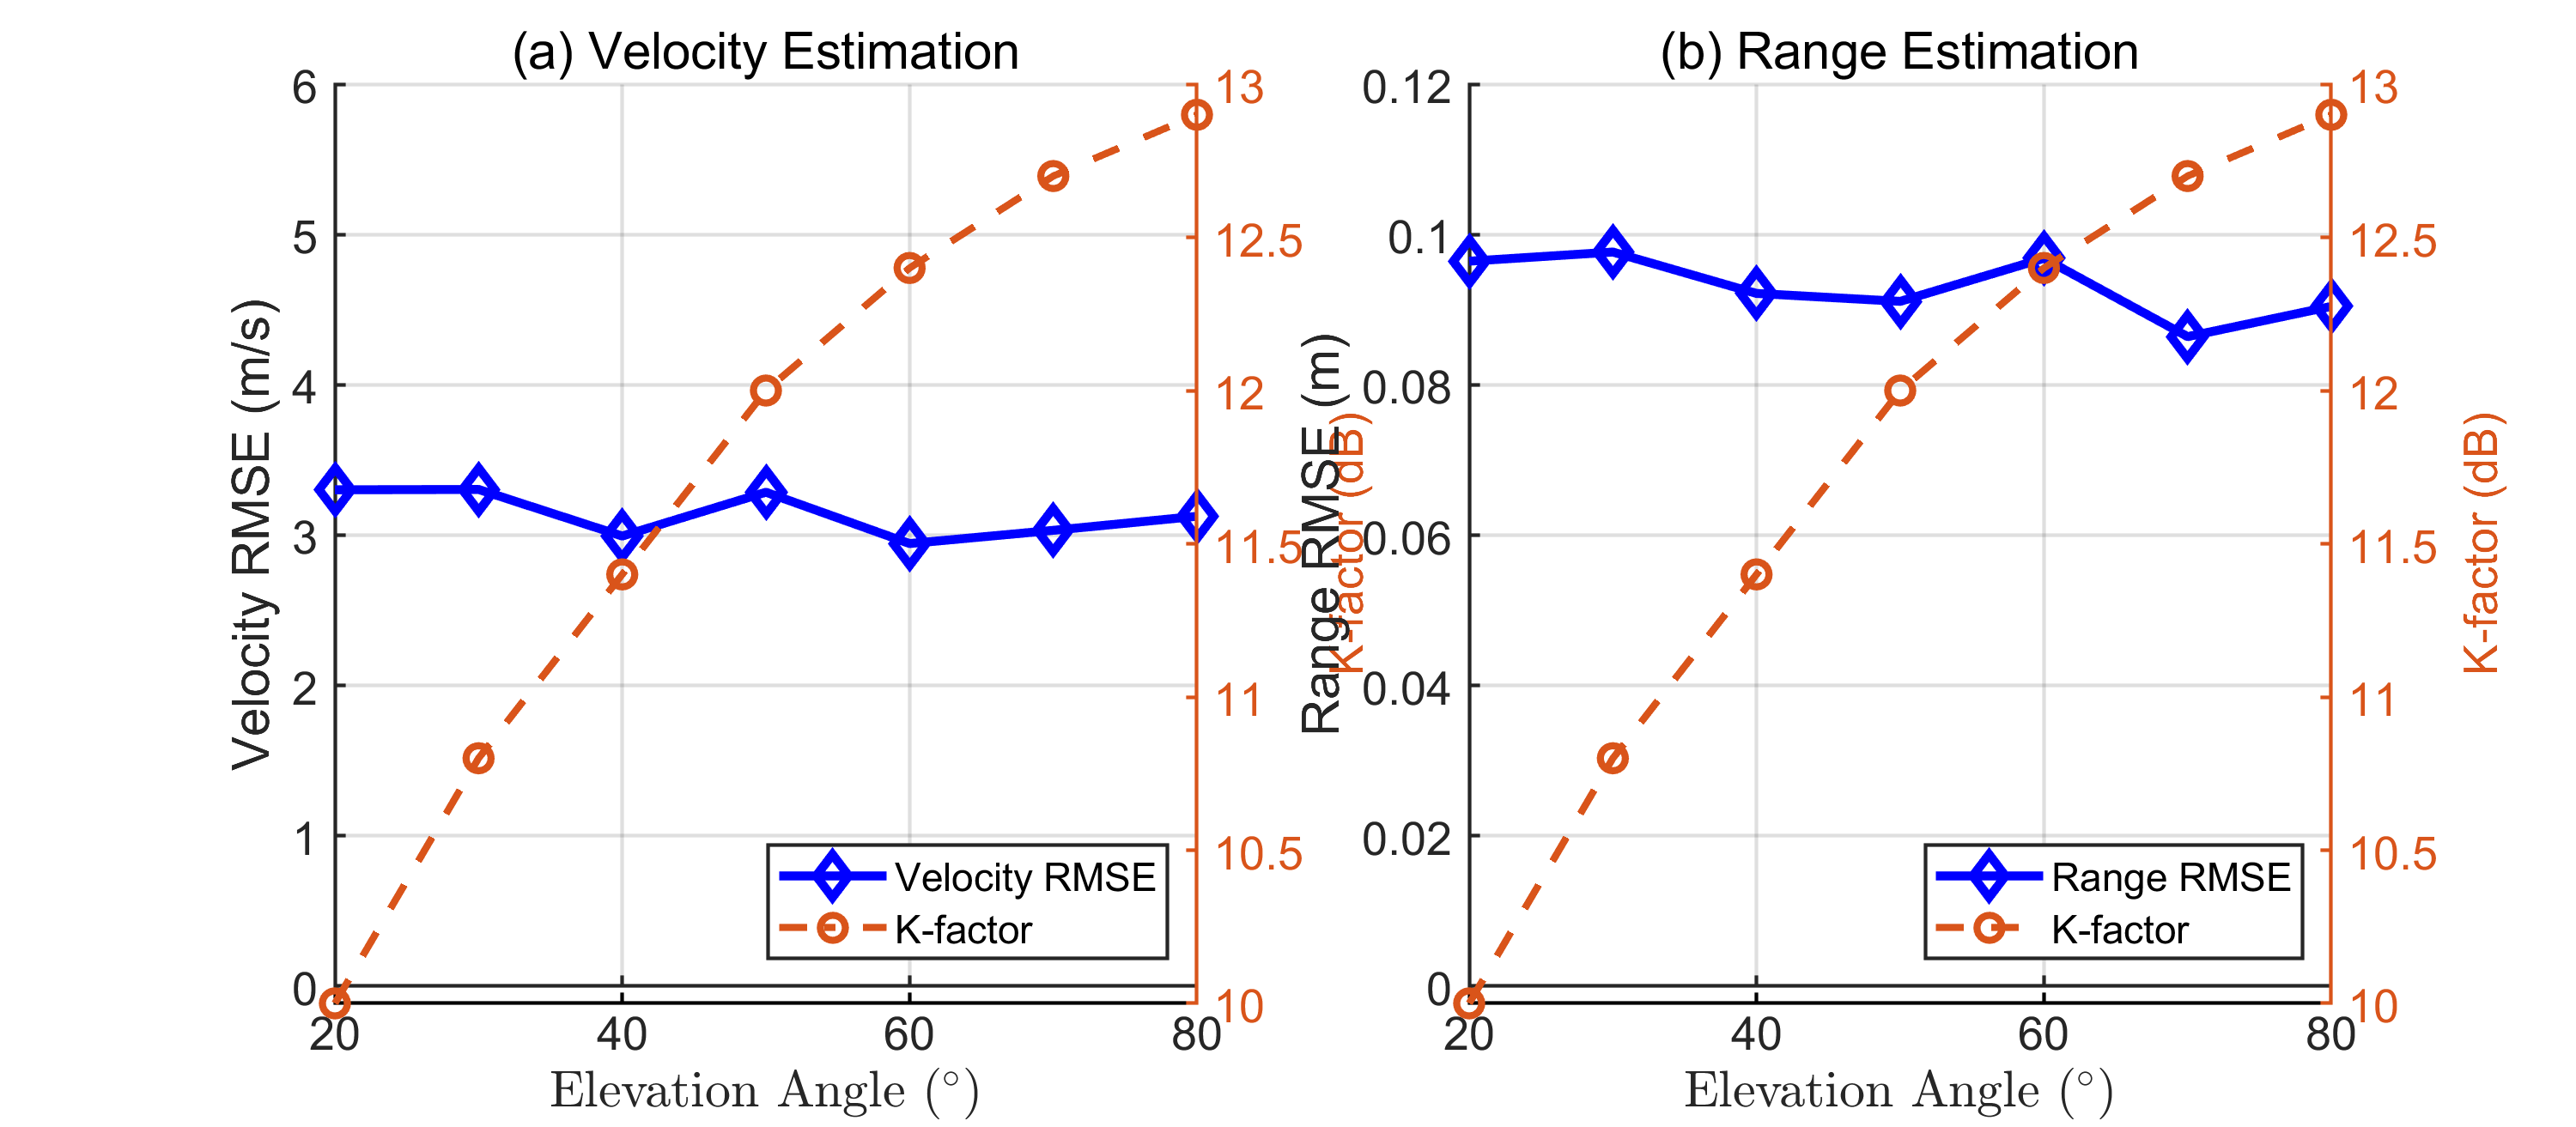
\includegraphics[width=\columnwidth]{../figure/SimulationResult/fig9_elevation_dependence.png}
  \caption{Navigation RMSE versus elevation angle, with the corresponding Rician K-factor shown on the right axis: (a)~velocity RMSE; (b)~range RMSE.}
  \label{fig:elev}
\end{figure}

Fig.~\ref{fig:elev} shows the effect of elevation angle through the associated Rician K-factor. As the elevation angle increases from $20^\circ$ to $80^\circ$, the K-factor rises from about $10$ to $12.9$~dB, while the navigation RMSE remains relatively stable: about $1.9$--$2.0$~m/s for velocity and $0.035$--$0.046$~m for range. Thus, the main observation is stability rather than monotonic gain.

%%=========================================================================
%%  V. CONCLUSION
%%=========================================================================
\section{Conclusion}

This paper presented a DD-domain impulse-pilot framework for OTFS-based ISAC in LEO NTN, targeting the extreme-Doppler regime in which conventional DD pilot placement becomes infeasible. Ephemeris-assisted Doppler pre-compensation reduces the required guard overhead to below $1\%$, and fractional-aware pilot reconstruction improves consistency between the DD channel model and the receiver processing chain. Simulations under the 3GPP NTN-TDL-C channel showed that OTFS-Ideal outperforms OFDM and OFDM-SIC in the high-SNR regime, while OTFS-Pilot preserves a substantial portion of this gain with practical channel estimation. The sensing results showed an approximately CRB-parallel trend, a clear advantage of fractional interpolation over integer-only estimation, robustness to moderate ephemeris error, and stable performance across elevation angles. Future work will consider stronger baselines, iterative multi-frame estimation, and experimental validation.

%%=========================================================================
%%  ACKNOWLEDGMENT
%%=========================================================================
\section*{Acknowledgment}
The author acknowledges the use of AI-assisted tools for English editing and manuscript formatting. All technical contributions and result interpretation were performed by the author.

%%=========================================================================
%%  REFERENCES
%%=========================================================================
\begin{thebibliography}{00}

\bibitem{3gpp_38811}
3GPP, ``Study on New Radio (NR) to support non-terrestrial networks,'' 3GPP TR~38.811 V15.4.0, 2020.

\bibitem{3gpp_38821}
3GPP, ``Solutions for NR to support non-terrestrial networks (NTN),'' 3GPP TR~38.821 V16.2.0, 2021.

\bibitem{wang_ofdm_ici}
T. Wang, J. G. Proakis, E. Masry, and J. R. Zeidler, ``Performance degradation of OFDM systems due to Doppler spreading,'' \textit{IEEE Trans. Wireless Commun.}, vol.~5, no.~6, pp.~1422--1432, Jun.~2006.

\bibitem{hadani2017otfs}
R. Hadani \textit{et al.}, ``Orthogonal time frequency space modulation,'' in \textit{Proc. IEEE WCNC}, Mar.~2017, pp.~1--6.

\bibitem{raviteja2018interference}
P. Raviteja, K. T. Phan, Y. Hong, and E. Viterbo, ``Interference cancellation and iterative detection for orthogonal time frequency space modulation,'' \textit{IEEE Trans. Wireless Commun.}, vol.~17, no.~10, pp.~6501--6515, Oct.~2018.

\bibitem{otfs_leo_2023}
J. Shi, Z. Li, J. Hu, Z. Tie, S. Li, W. Liang, and Z. Ding, ``OTFS enabled LEO satellite communications: A promising solution to severe Doppler effects,'' \textit{IEEE Netw.}, vol.~38, no.~1, pp.~203--209, Jan.~2024.

\bibitem{otfs_leo_jsac2025}
R. He, X.-F. Zhang, Q. Cui, and X. Tao, ``Doppler interference analysis for OTFS-based LEO satellite system,'' \textit{IEEE J. Sel. Areas Commun.}, vol.~43, no.~1, pp.~75--89, Jan.~2025.

\bibitem{dd_isac_2024}
W. Yuan, L. Zhou, S. K. Dehkordi, S. Li, P. Fan, G. Caire, and H. V. Poor, ``From OTFS to DD-ISAC: Integrating sensing and communications in the delay Doppler domain,'' \textit{IEEE Wireless Commun.}, vol.~31, no.~6, pp.~152--160, Dec.~2024.

\bibitem{gaudio2020otfs_radar}
L. Gaudio, M. Kobayashi, G. Caire, and G. Colavolpe, ``On the effectiveness of OTFS for joint radar parameter estimation and communication,'' \textit{IEEE Trans. Wireless Commun.}, vol.~19, no.~9, pp.~5951--5965, Sep.~2020.

\bibitem{raviteja2019}
P. Raviteja, K. T. Phan, and Y. Hong, ``Embedded pilot-aided channel estimation for OTFS in delay-Doppler channels,'' \textit{IEEE Trans. Veh. Technol.}, vol.~68, no.~5, pp.~4906--4917, May~2019.

\bibitem{loo_model}
C. Loo, ``A statistical model for a land mobile satellite link,'' \textit{IEEE Trans. Veh. Technol.}, vol.~34, no.~3, pp.~122--127, Aug.~1985.

\bibitem{3gpp_38901}
3GPP, ``Study on channel model for frequencies from 0.5 to 100~GHz,'' 3GPP TR~38.901 V17.0.0, 2022.

\bibitem{itu_p681}
ITU-R, ``Propagation data required for the design of earth-space land mobile telecommunication systems,'' Rec. ITU-R P.681-11, 2019.

\bibitem{quinn1997}
B. G. Quinn, ``Estimation of frequency, amplitude, and phase from the DFT of a time series,'' \textit{IEEE Trans. Signal Process.}, vol.~45, no.~3, pp.~814--817, Mar.~1997.

\bibitem{kay1993}
S. M. Kay, \textit{Fundamentals of Statistical Signal Processing: Estimation Theory}. Upper Saddle River, NJ: Prentice-Hall, 1993.

\end{thebibliography}

\end{document}


